\chapter{Analysis}
\minitoc
\label{Cap:Analysis}
%++++++++++++++++++++++++++++++++++++++
%     Introduction 
%++++++++++++++++++++++++++++++++++++++

tables only
\label{Cap:Analysis:Introduction}
In the \textbf{Subsection} \ref{Cap:Int:Motivation} the reasons to continue with the studies of the 1$\pi^+$ production in MINER$\nu$A experiment are explained. In this section, the process for the calculation of the one differential cross section (1D analysis) and a double differential cross section (2D analysis) for 1 pion production are shown. The results of the cross sections are shown in \textbf{Chapter} \ref{Cap:xSec}. The signal definition for both is the same. The innovation for these analyses is that two different techniques of data selection are used, these are explained in \textbf{subsections} \ref{Cap:Analysis:DataSelection:Cuts:Tracked} and \ref{Cap:Analysis:DataSelection:Cuts:UntrackedPions}. 

The measurement of the 1D analysis with respect to $x$ variable is obtained as follows:

\begin{equation}
    \left(\frac{d\sigma}{dx}\right)_i= \beta \frac{\Sigma_{j}U_{ij}(N^{data}_j - N^{simBkgd}_j)}{\epsilon_{i}\phi T\Delta x_i}
    \label{eq:difXSec}
\end{equation}

Where $j$ is the bin of the $x$ reconstructed variable, $i$ is the bin of the $x$ true variable, $N_j^{data}$ is the selected data for the reconstructed $j$ bin, $N_j^{sim Bkgd}$ is the simulated background for the reconstructed $j$ bin, $U_{ij}$ is the unfolding matrix, $\beta$ is the material correction factor, $\epsilon_i$ is the simulated efficiency of data selection and acceptance correction for the $i$ true bin, $\phi$ is the neutrino flux, $T$ is the number of target nuclei in the detector and $\Delta x_i$ is the bin width for the variable $x$ for the $i$ true bin.

For the case of the 2D analysis, with respect to the variable $x$ and $y$ is obtained as follows:

\begin{equation}
    \centering
    \left(\frac{d^2\sigma}{dxdy}\right)_{ij}= \beta \frac{\Sigma_{ab}U_{abij}(N^{data}_{ab} - N^{simBkgd}_{ab})}{\epsilon_{ij}\phi T\Delta x_{i}y_j}
\end{equation}

The measurement for the 2D analysis is similar to the 1D analysis, where $a$ and $b$ are the reconstructed bins for the $x$ and $y$ variables respectively, $i$ and $j$ are the true bins for the $x$ and $y$ variables respectively, $N_j^{data}$ is the selected data, $N_j^{sim Bkgd}$ is the simulated background, $U_{ij}$ is the unfolding matrix, $\beta$ is the material correction factor, $\epsilon_i$ is the simulated efficiency of data selection and acceptance correction, $\phi$ is the neutrino flux, $T$ is the number of target nuclei in the detector $\Delta x_i y_j$ is the bin width for the variable $x$ for the $i$ true bin.

In the way to compare the data, the MC models and the MC reconstruction simulation, there are three categories of data:
\begin{itemize}
    \item \textit{Data}: it corresponds to the reconstructed information obtained directly from the detector.
    \item \textit{MC}: It is the information obtained from the reconstructed interactions in the detector simulation, more details are given in \ref{Cap:MnvExp:MnvDetector:DataReconstruction}. 
    \item \textit{True}: it corresponds to the information obtained directly from the neutrino interaction simulation, it includes information obtained directly from the models, systematic errors of the models, particles ID, etc. More details in \ref{Cap:Simulation:GENIE}.
\end{itemize}

The information obtained from the \textit{MC} and \textit{true} data allows to simulate the background, to estimate the detector efficiency, to apply different cuts, to estimate the purity of the sample, to tune the background and compare the data directly with the models. 

In the following bullets are explained the steps to measure the cross section, for the 1D and 2D analysis cases:

\begin{enumerate}
    \item \textbf{Signal Definition and analysis variables:} This is the first stage of the analysis, in this stage is defined the physical process that will be studied. Here are studied the constrains for the analysis delimited by the detector capabilities and the variables respect to the differential cross section will be obtained. In the \textbf{sections} \ref{Cap:Analysis:SignalDefinition} and \ref{Cap:Analysis:Variables} are shown the specific signal definition and variables that will be used for the analyses. 

    \item \textbf{Data Selection:} At this stage, according to the signal definition, cuts are applied to the data set. To apply these cuts the data is passed event by event looking for characteristics that satisfy the requirements of the signal definition, at the same time the events that do not pass the cuts are removed. In the selected events set there are signal and background events. The signal events are the events that pass the cuts and satisfy the signal definition, by other hand the background corresponds to the events that pass the cuts but these do not correspond to the signal definition. From the MC simulation the signal and background events can be identify using the information obtained from the simulation process, but not in the data case. In this stage the simulated purity and efficiency are used to optimize the data selection. 

    The purity is calculated as follows:
    \begin{equation}
        purity=\frac{Signal\ Events}{Signal+Background\ Events}
        \label{eq:Analysis:Purity}
    \end{equation}
    The purity gives information about the fraction of the simulated data that actually corresponds to the signal definition. During the data selection process, it is essential to improve, remove, or apply cuts in the way to perform the data selection.

    For the efficiency, it is calculated as 
    
    \begin{equation}
        \epsilon=\frac{Signal\ Events}{True\ Signal\ Events}
        \label{eq:Analysis:efficiency}
    \end{equation}
    where the \textit{True Signal Events} corresponds to the total number of simulated events that match the signal definition. 
    In the \textbf{Section} \ref{Cap:Analysis:DataSelection} the results for the data selection are shown. 

    \item \textbf{Background subtraction:} In this step, the simulated background is removed from the data and MC data selection. One question about this procedure is how well is simulated the background, trying to have a better approximation to the real background in the experiment the \textit{Sideband} studies are developed to make the \textit{background tuning}. The sideband studies consist to apply the data selection but in phase space region where most part of the events are characterized to be background, it basically consist to remove one of the cuts that are applied during the data selection. In this region the simulation is fitted respect to the data. After to fit the background it is subtracted bin by bin to the data selection, giving as result the data selection histogram with out the background shape. 

    \item \textbf{Unfolding:} The detector is not perfect, there are many sources of uncertainties associated to the energy reconstruction, vertex reconstruction, particle identification, etc. These imperfections smear the data selection distributions. The unfolding procedure remove this smearing from the data selection. This can be interpreted as the unfolding transform the histogram from a reconstructed space to a true space where the detector is perfect. 

    \item \textbf{Efficiency correction:} During the data selection process there are events that do not pass the cuts because the inefficiency of the cuts. To repopulate the histograms with the lost events $\epsilon_i$ is used, $i$ is the true bin number. $\epsilon_i$ is obtained as in the \textbf{equation} \ref{eq:Analysis:efficiency} but for each bin. 

    \item \textbf{Normalization:} This is the last step on the cross section measurement, for this last part the efficiency corrected distributions are normalized by the number of protons and neutrons in the detector region (fiducial volume), the flux of neutrinos and the bin width to obtain the differential cross section. 
    
\end{enumerate}

    In the following sections present the results for each step of the differential and double differential cross section measurements. For these results, the data POT is 1.05689$\times 10^{21}$ and the MC POT is 4.37033$\times 10^{21}$.  The variables used for the analysis are described in the \textbf{Section} \ref{Cap:Analysis:Variables}.


\section{Analysis Variables}
\label{Cap:Analysis:Variables}

\subsection{One differential cross section}
\label{Cap:Analysis:Variables:1DAnalysis}

The differential cross section is obtained with respect to the variables presented in the \textbf{Table} \ref{tab:Analisys:AnaVariables:1Danalysis}. For some variables, the central value of the variable depends on if the event passes the cuts for a tracked pion or for a untracked pion. The cuts and the definitions for tracked and untracked pions are defined in the \textbf{Section} \ref{Cap:Analysis:DataSelection}.

\begin{table}[!htb]
    \centering
    \begin{tabular}{c|p{4.6in}}
        \hline
        Variable & Description \\ \hline
        $T_\pi$      & Pion kinetic energy. For this analysis the value of this variable is  obtained by two methods. These two methods are described in the \textbf{Section} \ref{Cap:Analysis:SignalDefinition}. \\ 
        \hline
        $\theta_\pi$ & Pion polar angle with respect to the neutrino beam direction. The central value of this variable depends on whether the event has a tracked or untracked pion. This is explained in the \textbf{Section} \ref{Cap:Analysis:DataSelection}. \\
        \hline
        $P_\mu$      & Muon momentum magnitude. The momentum of the muon is measured by the MINOS Near detector, and the muon momentum can be reconstructed by the track length or by curvature. The muon reconstruction is explained in \ref{Cap:MnvExp:MnvDetector:DataReconstruction}. \\
        \hline
        $\theta_\mu$ & Muon polar angle respect to the direction of the neutrino beam. This is measured by the MINER$\nu$A detector taking as origin the neutrino vertex position and the reconstruction algorithm measuring the angle.\\
        \hline
        $P^z_\mu$    & Muon longitudinal momentum respect to the neutrino beam. It is obtained by $P^z_\mu = P_\mu cos \theta_\mu$. \\
        \hline
        $P^T_\mu$    & Muon transversal momentum respect to the neutrino beam. It is obtained by $P^T_\mu = P_\mu sin \theta_\mu$. \\
        \hline
        $E_\nu$      & Neutrino energy. This is estimated by the relation $E_\nu = E_\mu + E_{had}$. Here $E_\mu$ is the muon energy and $E_{had}$ is the estimated hadronic energy. \\
        \hline
        $Q^2$        & Four-momentum transfer by the neutrino. Defined as $Q^2 = - (p_\nu -p_\mu)^2$ or using lepton kinematics $Q^2 = 2E_\nu(E_\mu-P^z_\mu) + m^2_\mu$. Here $p_\nu$ and $p_\mu$ are the four-momentum of the incoming neutrino and the muon, respectively.\\ 
        \hline
        $W_{exp}$    & Experimental invariant hadronic mass. $W_{exp} = m^2_N + 2m_NE_{had} - Q^2$ $= m^2_N + 2m_N(E_\nu-E_\mu)$ is used as an approximation of W.\\
        \hline
    \end{tabular}
    \caption{Variables used in the 1D analysis and a description of each variable.}
    \label{tab:Analisys:AnaVariables:1Danalysis}
\end{table}

These are some clarifications that have to be given for $E_{had}$ and $W_{exp}$. $E_{had}$ is a variable that usually is smeared fro the real value, it is because in the interactions that can be produced, can be produced, which are invisible to the detector. Other sources of smearing include the production of charged or neutral pions and the initial state of the nucleons. For this analysis the hadronic energy is obtained by two methods, depending if the event passes the cut to be a categorized as pion tracked or untracked event. For the case of the tracked event $E_{had}$ is obtained as follows:

\begin{equation}
    E_{had} = T_\pi + m_\pi + E_{had,\ no\ \pi^+}
    \label{eq:EhadTracked}
\end{equation}

Where $m_\pi$ is the rest mass of the positive pion, $E_{had,\ no\ \pi^+}$ is the  no-pion-muon corrected remaining energy. To obtain $E_{had,\ no\ \pi^+}$, the first step is to measure all the visible energy deposited by the final particles in the detector without the muon track energy. Usually called $E_{avail}$, then, the calorimetric energy from the pion candidate tracks is removed, and finally a calorimetric correction is applied, all this process is fully described in \cite{AaronThesis}.  

On the other hand, for the case where the event corresponds to an untracked pion event, the hadronic energy is calculated as follows: 

\begin{equation}
    E_{had} = N_{michels}m_\pi + E_{avail}
    \label{eq:EhadUntracked}
\end{equation}

Where $N_{michels}$ is the number of michel electrons observed, $m_\pi$ is the rest mass of the pion and $E_{Avail}$ is the available energy. This definition is made with the assumption that untracked pion events do not necessarily exhibit a pion track, although a pion is produced, hence the rest mass of the pion must be considered in the $E_{had}$ measurement. $E_{avail}$ is obtained as follows: 

\begin{equation}
    E_{avail} = \beta_{avail\ Scale}(E_{recoil\ Tracker} + E_{recoil\ ECAL)}
\end{equation}

where $\beta_{avail\ Scale}$ is a calorimetric scale that is always equal to 1.17, $E_{recoil\ Tracker}$ is the reconstructed energy in the tracker removing the muon deposited energy and the muon fuzz energy, the muon fuzz energy corresponds to the small tracks produced around the muon track, and the $E_{recoil\ ECAL}$ that corresponds to the energy reconstructed in the ECAL without the muon track and the muon fuzz energy.

The theoretical invariant mass (W) is calculated by $W^2=(p_\nu+p_N+p_\mu)^2$, where $p_\nu$, $p_N$ and $p_\mu$ are the neutrino, nucleon and muon four-moment, respectively. In the experiments $p_\nu$ and $p_N$ cannot be measured directly. However, in experiments $W_{exp}$ is commonly used as an approximation using variables that can be estimated. In this analysis to obtain $w_{exp}$ the two definitions of $E_{had}$ are used, it depends on the cuts that the event passes.  

\subsection{Double differential cross section}
\label{Cap:Analysis:Variables:2DAnalysis}

In a 2D analysis are combined 2 variables to have a more detailed description of the neutrino interactions. The combinations used for this analysis are $T_\pi$ vs $P_\mu$, $T_\pi$ vs $P^T_\mu$, $P^z_\mu$ vs $P^T_\mu$, and $E_\nu$ vs $T_\pi$.



%++++++++++++++++++++++++++++++++++++++
%     Signal definition 
%++++++++++++++++++++++++++++++++++++++

\section{Signal Definition}
\label{Cap:Analysis:SignalDefinition}

The signal definition delimits the physical process of interest for the analysis. Here, the interaction types and the space phase are defined depending on the detector capabilities.

Essentially, in this thesis the signal definition is the production of one charge pion events by muon-neutrino Charged Current interaction in the MINER$\nu$A tracker, writing in the condensed formula $CC\ \nu_\mu+CH\xrightarrow{}\pi^+ + X + \mu$. Where $CH$ corresponds to the plastic scintillator of the tracker, $\pi^+$ one positive charge pion, $X$ corresponds to a nucleon (proton or neutron) but not other mesons and $\mu$ that corresponds to the muon. There are other conditions that are not described in the condensed formula; these will be explained below. 

According to the physical progress defined above, the selected events must be produced by CC muon-neutrino interactions, producing only one charged pion without other mesons for a $W_{exp} <$ 1.4 GeV. $W_{exp}$ is limited with the intention to measure mainly events where $\Delta$ (1232) is produced, it also reduces multi-pion events, the production of neutral particles that cannot be detected directly and as $W_{exp}$ increases it is more difficult to measure the out coming particle kinematics. 

There are other limits applied to the signal definition due the detector capabilities, such as 1.5 GeV $<P_\mu<20$ GeV, $\theta_\mu<20$ GeV, vertex position in the MINER$\nu$A tracker region, and there are  different condition for $T_\pi$:
\begin{itemize}
    \item $0<T_\pi<350$ MeV, this condition is applied for the 1D analysis when $\theta_\pi$ is not included in the measurement.  
    \item $20<T_\pi<350$ MeV, this condition is applied for the 1D analysis when the variable $\theta_\pi$ is analyzed. 
\end{itemize}

The $T_\pi$ upper limit is imposed because the pions with a higher energy leave the detector and the pions cannot be reconstructed. The reason why there is a special signal definition for $\theta_\pi$ is because for the untracked pion events, $\theta_\pi$ is estimated by the polar angle between the neutrino direction and the position of the closest michel electron end point, using as reference the neutrino vertex interaction. This measurement is a good approximation to the real $\theta_\pi$ for a region of the pion kinetic energy; however, it is necessary to make an analysis of the region where the pion angle is not well reconstructed. In the \textbf{Figure} \ref{fig:Analysis:SignalDefinition:1DAnalysis:thetapivsTpi}. From the migration matrices, the discrepancy between the reconstructed and true $\theta_\pi$ is observed for the $T_\pi < 20$ MeV region. For this reason, it was decided to restrict $T_\pi$ only when $\theta_\pi$ is measured. 

The restriction for $P_\mu>1.5$ GeV is imposed because, below this momentum, the muon does not have enough momentum to reach the MINOS detector, and above 20 GeV the muon is going out of MINOS and the momentum cannot be measured by curvature. The restriction for $\theta_\mu < 20$\textdegree is due to the fact that it seeks to guarantee that the muon will leave MINER$\nu$A backward and enter the MINOS detector.

The analysis is focused to look for interactions in the tracker region, the fiducial volume defined for the Z axis in the detector coordinate system is 5990 cm $< z <$ 8340 cm with a transversal hexagonal area of 850 cm measured from the center of the detector. This region excludes the target upstream region, the downstream calorimeters, and the OD around the tracker region. 

For the 2D analysis, the signal definition is similar to the 1D analysis. For the 2D analysis, data selection does not include untracked pion events, and therefore $T_\pi$ is limited to the region 35 MeV $<T_\pi<$ 350 MeV. The lower limit is imposed because the tracked pions cannot pass through more than 5 planes; it is a reconstruction condition for the short tracks to be reconstructed. 


\begin{figure}[!htb]
    \centering
    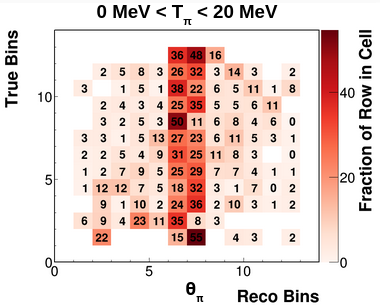
\includegraphics[scale=0.33]{Figures/Chapter4/SignalDefinition/thetapi0to20tpi.png}
    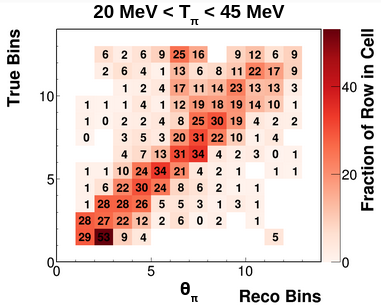
\includegraphics[scale=0.33]{Figures/Chapter4/SignalDefinition/thetapi20to45tpi.png}
    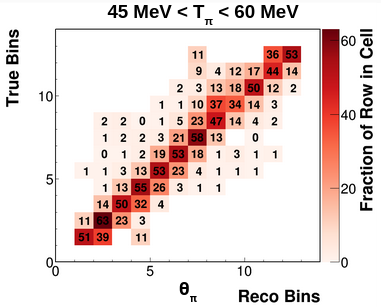
\includegraphics[scale=0.33]{Figures/Chapter4/SignalDefinition/thetapi45to60tpi.png}
    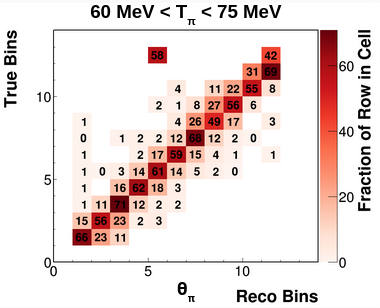
\includegraphics[scale=0.33]{Figures/Chapter4/SignalDefinition/thetapi60to75tpi.png}
    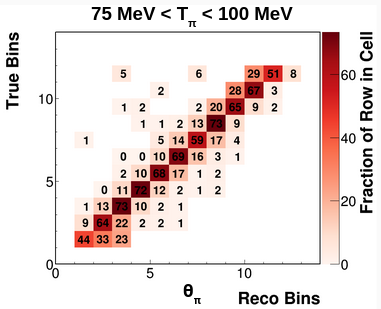
\includegraphics[scale=0.33]{Figures/Chapter4/SignalDefinition/thetapi75to100tpi.png}
    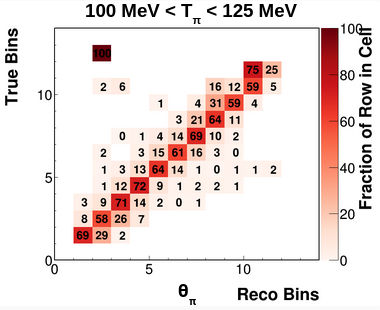
\includegraphics[scale=0.33]{Figures/Chapter4/SignalDefinition/thetapi100to125tpi.png}
    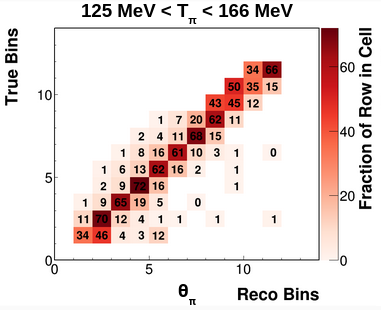
\includegraphics[scale=0.33]{Figures/Chapter4/SignalDefinition/thetapi125to166tpi.png}
    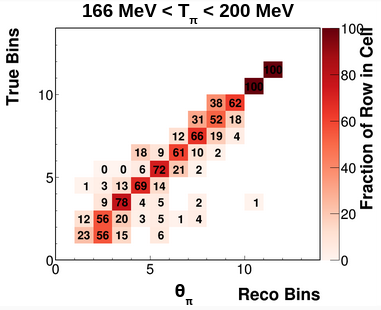
\includegraphics[scale=0.33]{Figures/Chapter4/SignalDefinition/thetapi166to200tpi.png}
    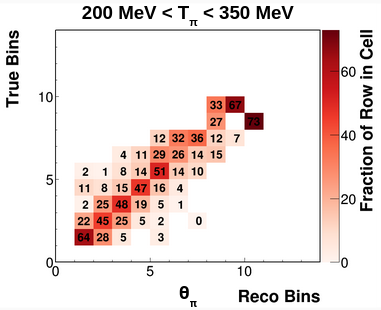
\includegraphics[scale=0.33]{Figures/Chapter4/SignalDefinition/thetapi200to350tpi.png}
    \caption{Migration matrices for $\theta_\pi$ for different regions of True $T_\pi$. The bad reconstruction of $\theta_\pi$ for $0<t_\pi<20$ MeV is shown. The $\theta_\pi$ binning showed in the plots does not correspond to the real binning, it just a homogeneous binning used to have a better perception of the migration matrix. The $\theta_\pi$ binning used for this analysis is [0., 15., 30., 45, 60, 75., 90., 105., 120., 135., 150., 165., 180.].}
    \label{fig:Analysis:SignalDefinition:1DAnalysis:thetapivsTpi}
\end{figure}


%++++++++++++++++++++++++++++++++++++++
%     Data Selection 
%++++++++++++++++++++++++++++++++++++++
\section{Data Selection}
\label{Cap:Analysis:DataSelection}

In this section are described the cuts that are applied to obtain the data selection for the 1D and 2D analyses. Here are shown the cut tables for the events that pass the cuts, showing the efficiency and purity of the data selection. The signal definition described in the \textbf{Section} \ref{Cap:Analysis:SignalDefinition} delimit what kind of events should be included in data selection. In data selection, the quantities that must be optimized are the purity and the efficiency. The way to increase the purity is to increase the cuts or restrictions applied to the data set, but it reduces the efficiency of data selection at the same time that increases the statistical error. 

In particular, this analysis uses two different data selection techniques, which are named tracked pion data selection and untracked pion data selection. The reasons for this mixed data selection are explained in \ref{Cap:Int:Motivation}.


\subsection{Cuts}
\label{Cap:Analysis:DataSelection:Cuts}

Cuts are classified into three types. The \textit{General cuts}, \textit{tracked Pion cuts} and the \textit{Untracked Pion cuts}. The general cuts are applied to the tracked and untracked pion events. The general cuts are as follows.

\begin{itemize}
    \item \textbf{Vertex position Cut}: This cut removes all the events where the interaction vertex is no produced in the fiducial volume defined in the signal definition. In this analysis, the interaction must be produce in the tracker region. 
    \item \textbf{Muon Cuts}: In signal definition it is required that the incident neutrino must have a muon-neutrino and it have to interact by Charged Current interaction, for this reason the events must to have an observable muon track and it also has to reach the MINOS detector and produce a muon with a curvature that corresponds to a negative muon. This cut remove the Neutral Current (NC) interaction events and the muon charge sign removes the events that are coming from $\overline{\nu_\mu}$. 
    
    The other muon cuts remove the events where the reconstructed muon has $\theta_\pi<$ 20\textdegree and when $P_\mu < 1.5$ GeV and $P_\mu>$ 20 GeV, the reasons why these cuts are applied are the same as the conditions imposed in the signal definition.  
    \item \textbf{$\pi^0$ Cut}: This cut removes the events where $\pi^0$ are produced. The $\pi^0$ cannot be observed directly; however, these decay very fast, producing two gammas. In the detector it is observed as isolated energy clusters generated out of the vertex interaction position with a time limit of \(\sim\) 30 ns after the neutrino interaction. This cut increases the purity around of 9\% and has a cut efficiency of 95\%. 
\end{itemize}


\subsubsection{Tracked pions}
\label{Cap:Analysis:DataSelection:Cuts:Tracked}

These are the cuts typically applied in the charge pion analyses in the \textbf{Section} \ref{Cap:Int:Motivation}. For this analysis, most of the cuts are applied and these are described in the following bullets. 

\begin{itemize}
    \item \textbf{At least one hadron track:} At least one track that does not correspond to the muon track must be observed in the vertex. These tracks are considered as candidate hadron tracks and must undergo the hadron quality cuts. The hadron track quality cuts check whether the hadron track is forked, exiting, produced in the side ECAL, matches the OD, and is produced in the tracker. The Forked cut is impose to remove the events where the hadron interacts with the detector creating other tracks making it difficult to measure the hadron energy. The exiting cut removes the events where the hadron track is not contained in the ID region, hence is not possible to measure the total hadron energy. The side ECAL matches the OD cuts removes the events where hadron is going to the side ECAL or to OD. The last cut, checks if the reconstructed hadron is contained in the tracker.
    \item \textbf{At lest 1 matched michel electron:} The 99.9\% of the $\pi^+$ decays in the way $\pi^+\xrightarrow{}\mu^+ + \nu_\mu$ with a life time of $\tau \sim$ 26 ns, after the $\mu^+$ decays as $\mu^+\xrightarrow{} e^+ + \overline{\nu}_\mu + \nu_e$ with a life time $\tau\sim$ 2.2 \(\mu\)s, the $e^+$ produced is known as michel electron. The michel electron is observed as a track spatial separated and time-delayed from the interaction neutrino vertex. 

    Based on the previous description of the michel electrons, the selection of the michel electrons is performed by initially searching for hit clusters produced in time slices after the neutrino interaction. The distance between the vertex and the cluster must not exceed 50 cm, and the energy of the michel electron must be consistent with the energy expected from the muon decay process.  

    \begin{figure}[!htb]
        \centering
        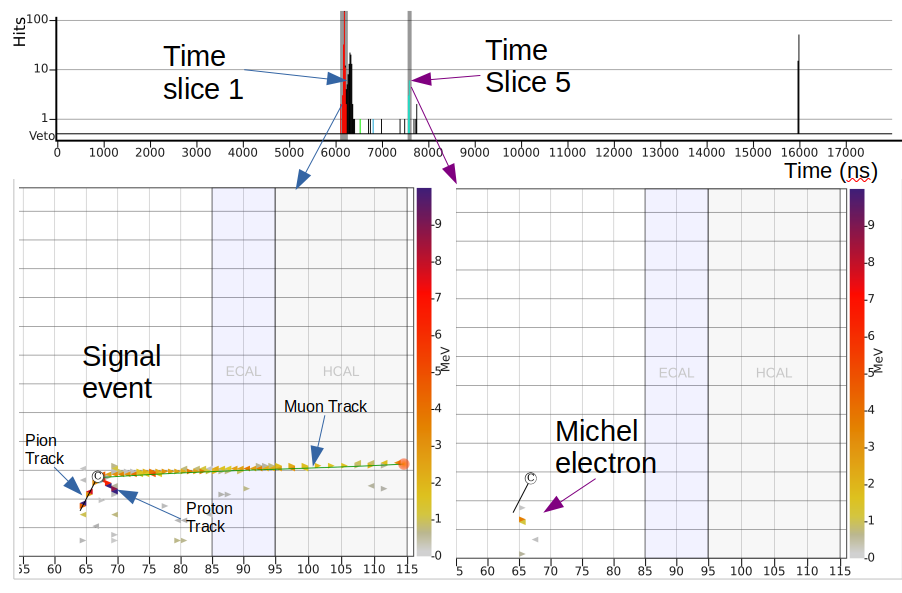
\includegraphics[scale=0.4]{Figures/Chapter4/DataSelection/EventDisplayMichelElectronRun110000SubRun146.png}
        \caption{Event display of a MC event for a tracked pion for the the run 110000, subrun146, Gate 1 for the XZ view. This figure shows and simulated signal event for the time slice 1 (left) and the time slice 5 (right). This shows an event where the michel electron is found. }
        \label{fig:Analysis:DataSelection:Cuts:Tracked:EventDisplayMETracked}
    \end{figure}

    The next step is to associate the michel electron with a hadron track. The first step is to measure the distance between the michel electron and the endpoint of the hadron track. The subsequent step involves categorizing the michel electron into the following types: \textit{fitted}, \textit{Unfitted}, and \textit{One-view}. The michel electron's category depends on the number of detector planes it traverses. A michel electron falls into the fitted category when it passes through multiple planes, and its track can be reconstructed as a line. For this category, the distance is measured between the endpoint of the hadron track and the closest endpoint of the michel electron track. In the case of the unfitted category, the michel electron passes through at least two planes. For this case, the distance is measured from the endpoint to the cluster's energy-average mean position. In the last case, the michel electron falls into this category when it only deposits energy in just one plane, and the distance is measured similarly to the unfitted category. 

    Depending of the category, the maximum distances are imposed, for the fitted = 7.5 cm, the unfitted = 50 cm and the one-view = 50 cm. In the cases of multiple hadron tracks it takes closer candidate to the michel electron, giving a pion candidate.
    


    
    \item \textbf{Particle Identification (PID) score:} After to get the pion candidate, the PID cut removes the events where the track is confused and it does not correspond to a pion-like track profile.
    
    During the reconstruction process, the algorithm initially identifies the muon track and assumes that the remaining tracks correspond to either a proton or a charged pion. To each track is estimated the energy-loss per unit of length of the charged particle when it pass through matter, more commonly know as $\frac{dE}{dx}$. These $\frac{dE}{dx}$ are compared with the $\frac{dE}{dx}$ profile of a proton and a charge pion, obtained by the Bethe-Bloch formula \cite{DetectionTechniques}. Each particle has a particular $\frac{dE}{dx}$ profile. The MINER$\nu$A Bethe-Bloch curves for the proton and pion are shown in the \textbf{Figure} \ref{fig:Analysis:DataSelection:Cuts:dEdXBetheProfiles}. 


    \begin{figure}[!htb]
        \centering
        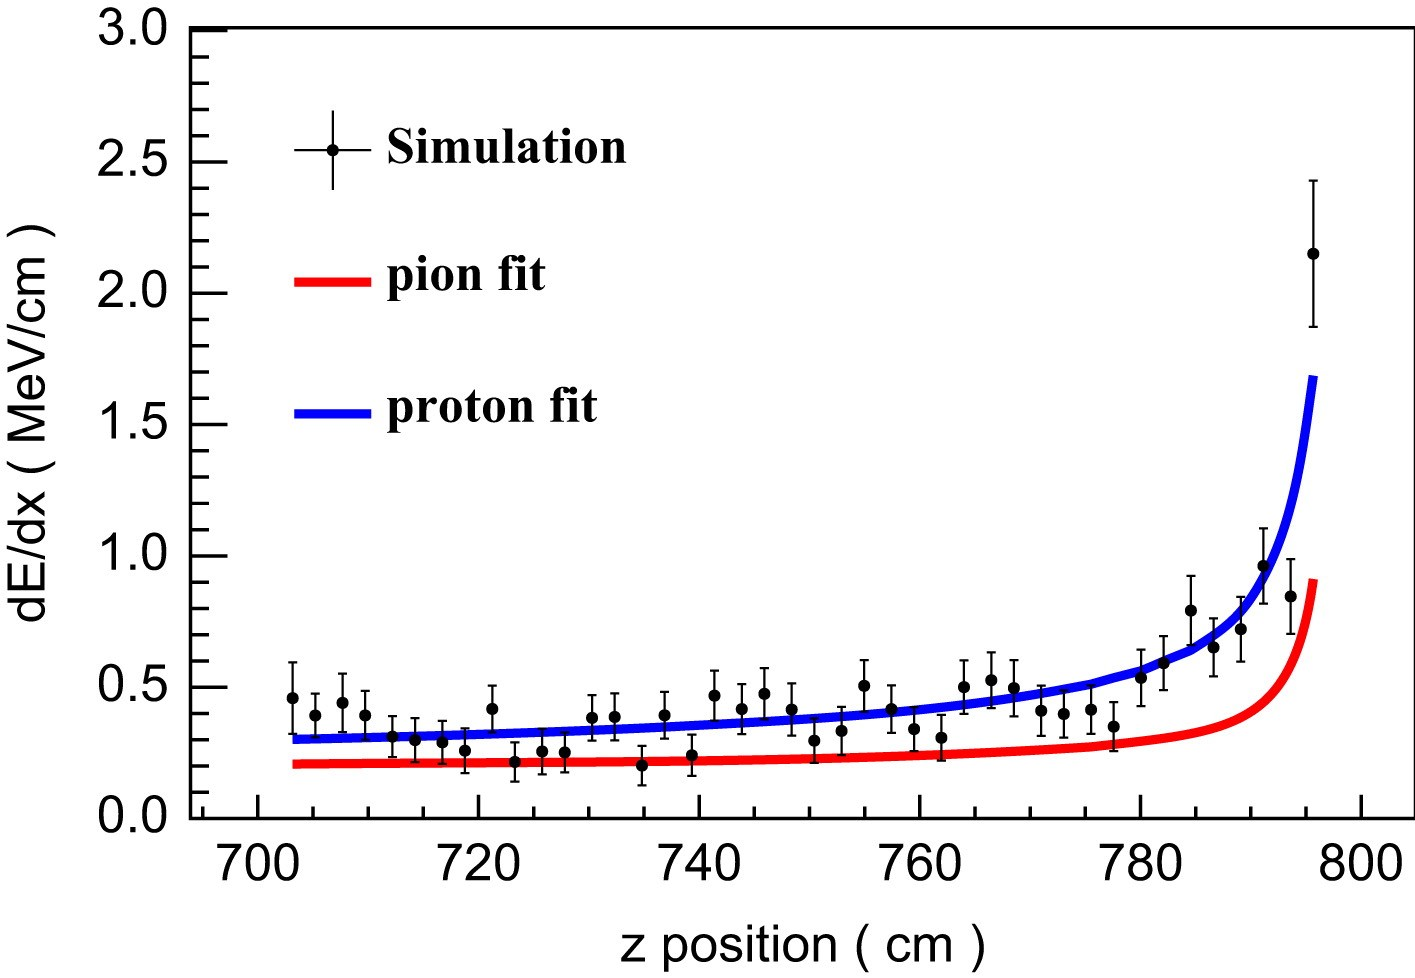
\includegraphics[scale=0.1]{Figures/Chapter4/DataSelection/dedxprotonSim.jpg}
        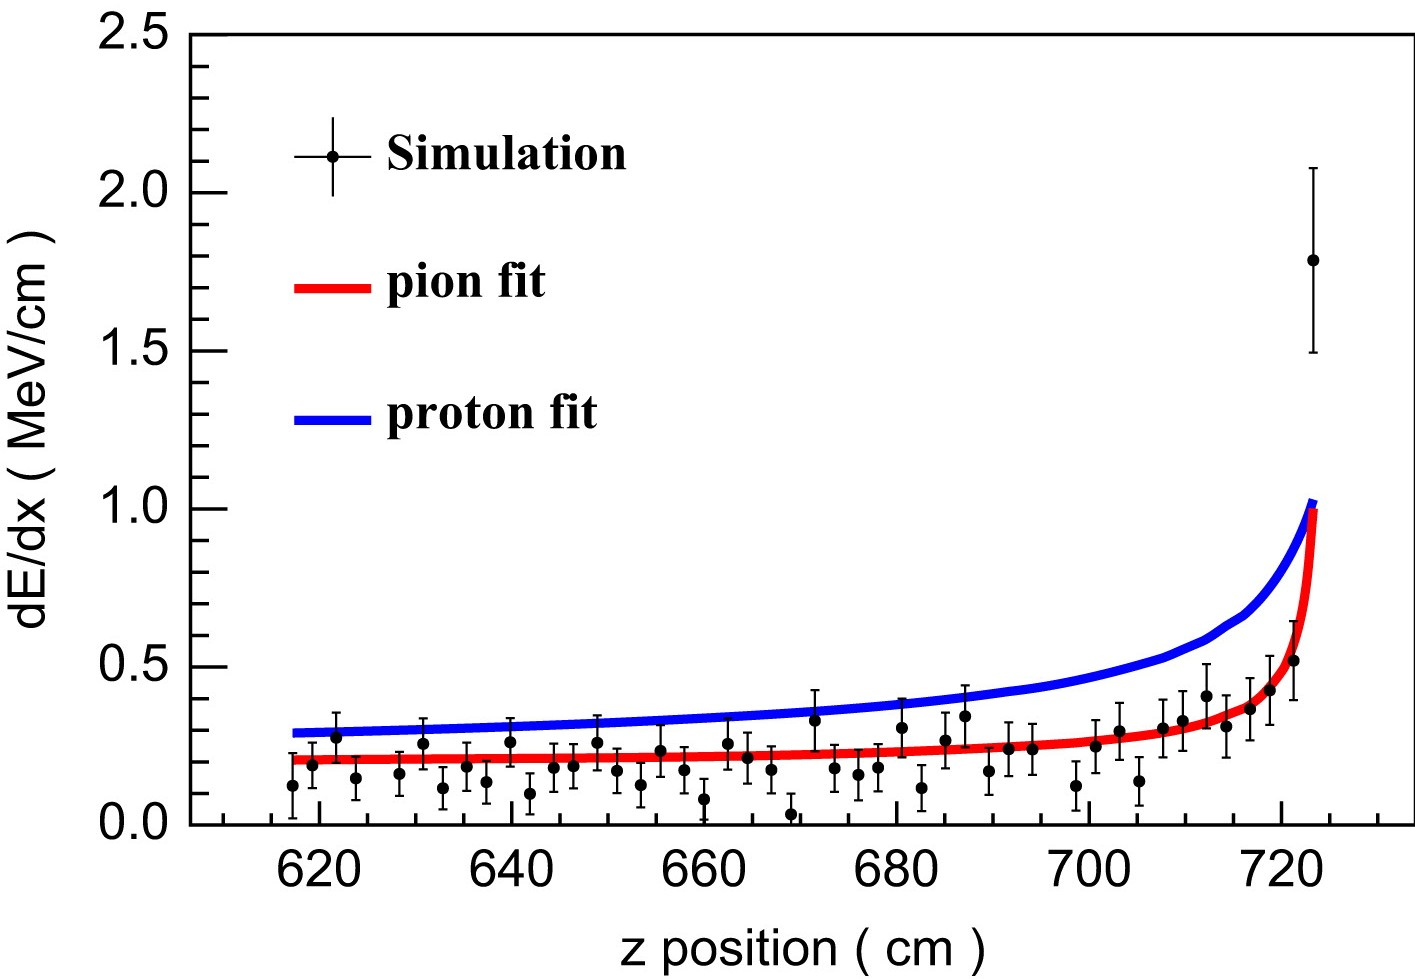
\includegraphics[scale=0.1]{Figures/Chapter4/DataSelection/dedxpionSim.jpg}
        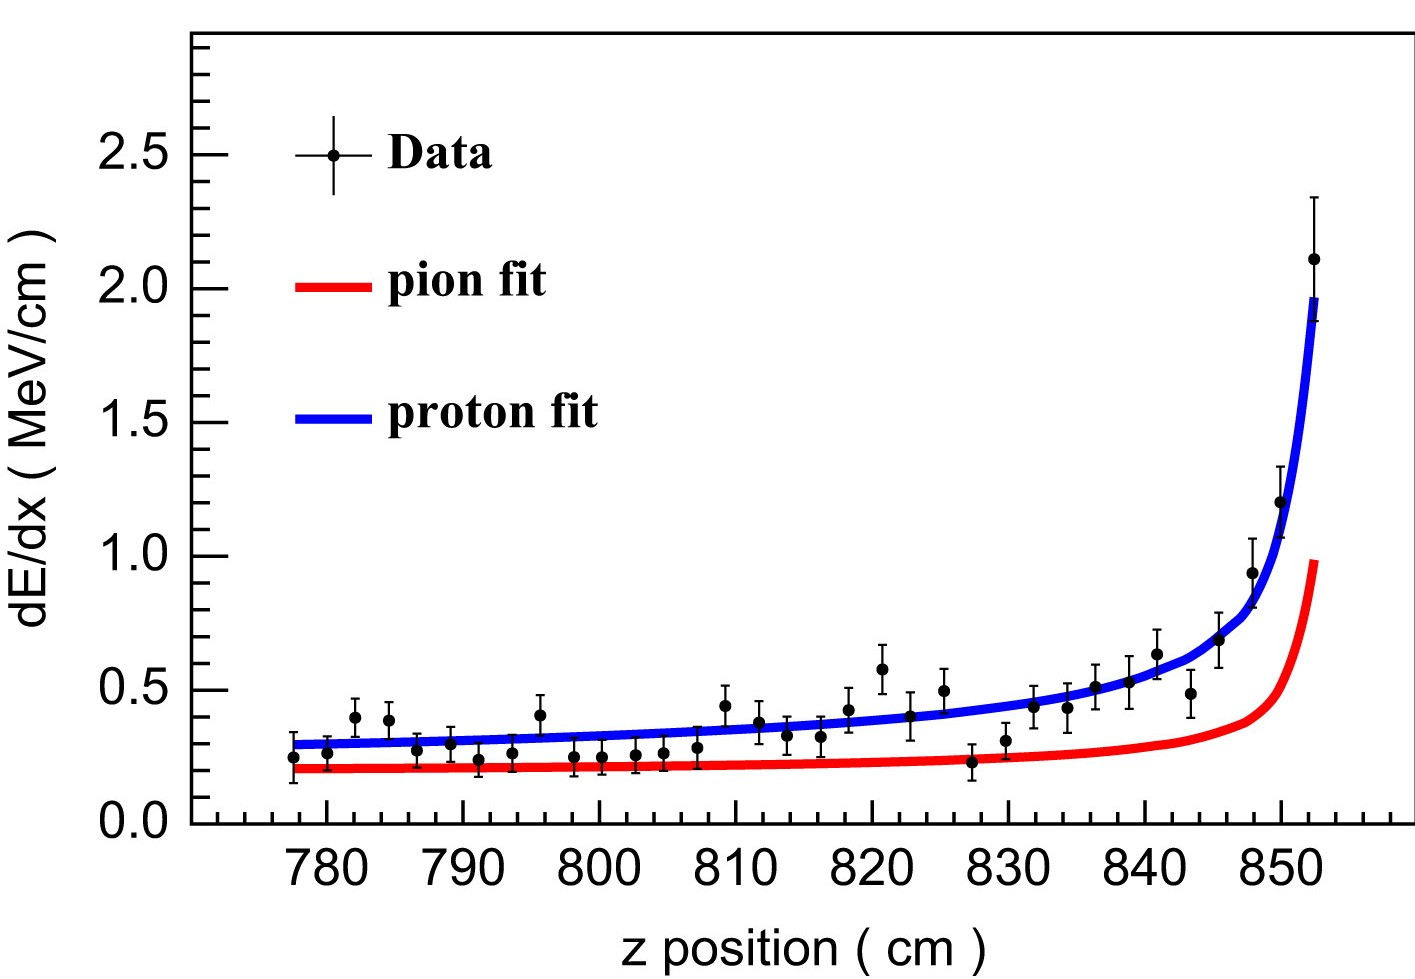
\includegraphics[scale=0.1]{Figures/Chapter4/DataSelection/dedxprotonData.jpg}
        \caption{The plots show the comparison of the Bathe-Bloch $\frac{dE}{dx}$ profiles for protons and pions with the simulated $\frac{dE}{dx}$ profiles for protons (top-left), pions (top-right) and for data taken using protons (bottom). Figures taken from \cite{MINERvA}.}
        \label{fig:Analysis:DataSelection:Cuts:dEdXBetheProfiles}
    \end{figure}

    To obtain the PID score of a track, each node of the track is compared with a likelihood function template that was created using a large set of simulated protons and pions. This was done using a Monte Carlo (MC) gun, varying the angle and energy of the particles. The likelihood template calculates the probability by assessing the fraction of pion or proton tracks with a node of identical energy at the same position along the track. The likelihood function $\mathcal{L}$ is formed as the product of all these individual probabilities as follow:
    \begin{equation}
        \mathcal{L}\left(particle|track\right)=\prod_{Nodes}P\left(E_{Node}|particle\right)
    \end{equation}

    Using the log of the Neyman-Pearson lemma \cite{Neyman-Pearson} to obtain the most optimal criteria to distinguish between the particle hypothesis, called the PID score, is obtained by

    \begin{equation}
        PID\ Score = \sum_{Node} (logP(E_{node}|\pi)-logP(E_{node}|p))
        \label{eq:Analysis:Cuts:PID}
    \end{equation}

    For the cases where there are overlapped tracks close to the interaction vertex, the PID score is not a reliable metric, for this reason when it is observed that in a track the energy in a node falls more than 1.9737 MeV between two nodes in the first 10 nodes the high-energy nodes are removed from the PID calculation. The Bethe-Bloch equations assume that the particles are stopped in the material, which means that the particle does not interact inelastically with the material. For this reason in the likelihood calculation these effects are included and the maximum likelihood is used. 

    This analysis is focused on pion, hence in the \textbf{Equation} \ref{eq:Analysis:Cuts:PID} the PID score $>$ 0 corresponds to a major probability that track corresponds to a pion. 

    
    \item \textbf{End nodes energy:} This cut is used to remove the events where the pion candidate interacts with the detector inelastically, because the energy usually is not well reconstructed for this kind of events. A bad reconstruction of this quantity implies a bad reconstruction of other variables such as $E_\nu$, $W_{exp}$ and $Q^2$. 

    When a particle travels through matter, it loses energy by ionization radiation, the $\frac{dE}{dx}(x)$ presents a pronounced peak before the particle comes to rest. This peak is known as the Bragg peak \cite{BraggCurves}. It must to be observed as increase of deposited energy at the end of the hadron track. 

    For the cases where the particle interacts inelastically with the detector, the Bragg peak is not observed. Therefore, events in which the candidate for the pion does not exhibit the Bragg peak are excluded from the data selection. The Bragg peak for the proton presents a higher increase increase compared with the peak generated by a pion, therefore, this cut also applies an upper limit removing events where the chosen track does not correspond to a pion. 

    This cut checks the deposited energy in the last 6 nodes of the pion candidate track. The \textbf{Table} \ref{tab:Analysis:Cuts:EndnodeCuts} shows the energy ranges per end-node that the pion candidate track must have.  

    \begin{table}[]
        \centering
        \begin{tabular}{c|c}
            End Node & Energy Range (MeV)\\ \hline
            0+1      & (6, 32) \\
            2        & (2, 22) \\
            3        & (0, 19) \\
            4        & (0, 31) \\
            5        & (0, 60) \\
        \end{tabular}
        \caption{Acceptable ranges for last nodes of the end of each track.}
        \label{tab:Analysis:Cuts:EndnodeCuts}
    \end{table}

    
    \item \textbf{Pion Multiplicity:} This cut removes the events where there more that 1 pion track candidate. This cut also removes the events where $T_\pi < 35$ MeV and $T_\pi > 350$ MeV. 
    \item \textbf{$W_{exp}$ tracked cut:} This cut removes all the event that have an $W_{exp} > 1.4$ GeV. The reasons why this cut is applied are already explained in the signal definition \ref{Cap:Analysis:SignalDefinition}. The measurement of $W_{exp}$ requires $E_{had}$, for this cut is used the $E_{had}$ obtained by the procedure explained in \ref{Cap:Analysis:Variables} for the tracked pions. 
    
\end{itemize}

In \ref{tab:Analysis:Cuts:TrackedCutTable1} and \ref{tab:Analysis:Cuts:TrackedCutTable2} the cut tables for the tracked pions are shown. In these cut tables only, the tracked pion efficiency and purity are shown. This table was obtained using only the ME1A playlist from the MINERvA data set. In the tables, the general cuts are applied as well. 

\begin{table}[!hbt]
    \tiny
    \centering
    \begin{tabular}{|*{7}{l|}}


    \hline
    & \multicolumn{4}{c|}{Signal} & \multicolumn{2}{c|}{Background} \\
    \hline
& N     & Eff     & Cut Eff & Pur    & N         & Eff  \\\hline

 No Cuts   & 203952.17     & 100.00\% & 100.00\% &   1.12\% & 17978780.42 & 100.00\% \\ \hline
 Anatool Precuts   & 159558.28     &  78.23\% &  78.23\% &   5.62\% & 2677126.18 &  14.89\%  \\ \hline
 vertex position Cut   & 156840.33     &  76.90\% &  98.30\% &   5.79\% & 2551834.64 &  14.19\%  \\ \hline
 MINOS Muon   & 151236.27     &  74.15\% &  96.43\% &   9.77\% & 1396389.62 &   7.77\%  \\ \hline
 1.5 GeV $<$ Pmu $<$ 20 GeV   & 150525.85     &  73.80\% &  99.53\% &  10.12\% & 1336621.79 &   7.43\%  \\ \hline
 $\theta_{\mu}$ $<$ 20 degrees   & 150457.23     &  73.77\% &  99.95\% &  10.30\% & 1310983.53 &   7.29\%  \\ \hline
 $<$2 Isolated Prongs   & 134544.17     &  65.97\% &  89.42\% &  17.94\% & 615463.26 &   3.42\%  \\ \hline
 $>$= 1 Hadron Track   & 77042.84     &  37.77\% &  57.26\% &  21.07\% & 288531.88 &   1.60\% \\ \hline
 $>$= 1 Michel   & 25370.23     &  12.44\% &  32.93\% &  42.89\% & 33787.16 &   0.19\% \\ \hline
 LLR PID   & 19359.43     &   9.49\% &  76.31\% &  45.58\% & 23117.93 &   0.13\% \\ \hline
 Node   & 15028.78     &   7.37\% &  77.63\% &  50.04\% & 15005.18 &   0.08\% \\ \hline
 Pion Multiplicity   & 15027.89     &   7.37\% &  99.99\% &  50.18\% & 14920.42 &   0.08\% \\ \hline
 $Tracked W_{exp}$   & 13709.32     &   6.72\% &  91.23\% &  67.31\% & 6657.79 &   0.04\% \\ \hline
    \end{tabular}
    \caption{Cut table for tracked events (Part 1). DataPOT: 89785235631482617856.00. MCPOT: 406599660544667287552.00.}
    \label{tab:Analysis:Cuts:TrackedCutTable1}
\end{table}

\begin{table}[!hbt]
    \tiny
    \centering
    \begin{tabular}{|*{6}{l|}}


    \hline
    & \multicolumn{2}{c|}{Total} & \multicolumn{3}{c|}{Data} \\
    \hline
&  N         & Eff     & N MC (scale) & N Data    & Data/MC \\\hline

 No Cuts   & 18182732.59 & 100.00\% & NA & NA & NA \\ \hline
 Anatool Precuts & 2836684.46 &  15.60\% & NA & NA & NA \\ \hline
 vertex position Cut   & 2708674.97     &  14.90\% & 598128.93     & 676952.00 &   1.13 \\ \hline
 MINOS Muon  & 1547625.89     &   8.51\% & 341746.36     & 358090.00 &   1.05 \\ \hline
 1.5 GeV $<$ Pmu $<$ 20 GeV   & 1487147.65     &   8.18\% & 328391.57     & 342163.00 &   1.04 \\ \hline
 $\theta_{\mu}$ $<$ 20 degrees   & 1461440.76     &   8.04\% & 322714.99     & 335784.00 &   1.04 \\ \hline
 $<$2 Isolated Prongs   & 750007.43     &   4.12\% & 165616.45     & 173567.00 &   1.05 \\ \hline
 $>$= 1 Hadron Track  & 365574.72     &   2.01\% & 80726.12     & 82223.00 &   1.02 \\ \hline
 $>$= 1 Michel   & 59157.39     &   0.33\% & 13063.12     & 12876.00 &   0.99 \\ \hline
 LLR PID  & 42477.35     &   0.23\% & 9379.84     & 9141.00 &   0.97 \\ \hline
 Node  & 30033.96     &   0.17\% & 6632.09     & 5991.00 &   0.90 \\ \hline
 Pion Multiplicity   & 29948.32     &   0.16\% & 6613.18     & 5984.00 &   0.90 \\ \hline
 $Tracked W_{exp}$  & 20367.11     &   0.11\% & 4497.46     & 4055.00 &   0.90 \\ \hline
    \end{tabular}
    \caption{Cut table for tracked events (Part 2). DataPOT: 89785235631482617856.00. MCPOT: 406599660544667287552.00.}
    \label{tab:Analysis:Cuts:TrackedCutTable2}
\end{table}


\pagebreak

\subsubsection{Untracked pions}
\label{Cap:Analysis:DataSelection:Cuts:UntrackedPions}
The implementation of these cuts aims to increase the efficiency of the data sample, expanding the $T_\pi$ range without compromising purity. This data selection is grounded in the observation that 99\% of charged pions decay to produce a muon, which subsequently emits a Michel electron. With this in mind, it becomes feasible to identify pions by counting the number of Michel electrons generated after the neutrino interaction, even in the absence of a discernible pion track. Assuming that the muon produced by the pion decay travels in the same direction as the primary pion and that the distance between the Michel electron and the vertex is correlated with $T_\pi$, it becomes possible to mitigate the dependency on the pion candidate track having a new data selection. 

To understand the data selection process, it is important to define the following quantities:
\begin{itemize}
    \item \textbf{Interaction vertex}: It corresponds to the position of the neutrino interaction reconstructed in the 3D space. 
    \item \textbf{Michel Cluster}: These are the clusters that are produced as time slices after the neutrino interaction. The michel cluster endpoint has to be well reconstructed. 
    \item \textbf{Closest Michel endpoint:} For the michel cluster two endpoints must be produced. The distance between the vertex and these endpoints is measured, and then the closest endpoint is selected.
    \item \textbf{Pion range:} It is the 3D distance between the interaction vertex and the closest endpoint.
    \item \textbf{Non-muon cluster:} this is a reconstructed cluster that is not associated with a muon. It could be a pion, proton, or other charged particle track. 
\end{itemize}
\begin{figure}
    \centering
    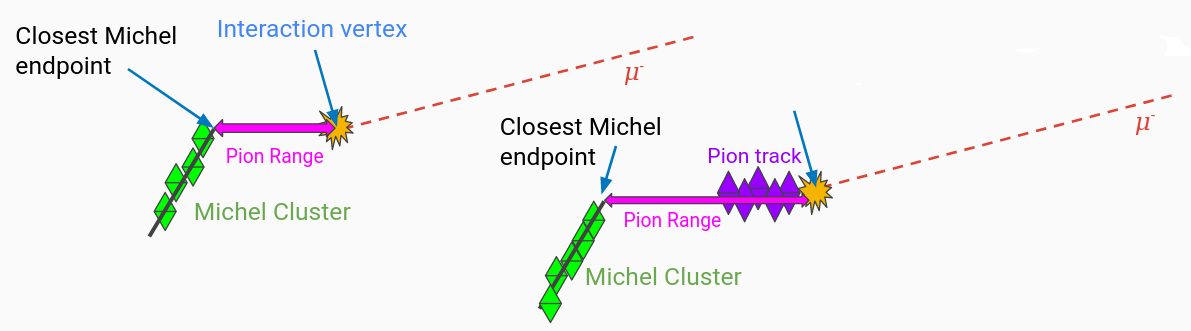
\includegraphics[scale=0.33]{Figures/Chapter4/DataSelection/TracklessPions.png}
    \caption{Scheme with two examples of pion events that can be produced part of the data selection, in the left, an event where the pion track is no produced but a michel electron is observed. The right scheme, it shows an event where is produced the track of a pion. }
    \label{fig:Analysis:Cuts:Untracked:MichelEventSheme}
\end{figure}

The cuts applied for the trackless pion are:

\begin{itemize}
    \item \textbf{Fitted Michel:} This cut eliminates all events where the Michel electron cluster is not reconstructed as fitted. As described earlier, Michel electron clusters fall into the fitted category when they traverse multiple planes, and the endpoints of the Michel electron are well reconstructed. Instances where unfitted or one-view Michel electrons are observed are excluded from the selection. Additionally, this cut removes Michel electrons that are observed 400 ns after the neutrino interaction. The output of this cut includes the identified Michel electron candidates.

    \item \textbf{2D distance cut:} The 2D distance cut measures the distance between vertex and michel electron ($XZ_{vtx-e}$, $UZ_{vtx-e}$ or $VZ_{vtx-e}$) or non-muon cluster  and michel electron ($XZ_{cluster-e}$, $UZ_{cluster-e}$ or $VZ_{cluster-e}$) for each michel endpoint. If the the distance exceeds 150 mm in 2 views the michel does not pass the cut. 
    
    The distance between the two views with respect to the vertex is obtained as follows: \begin{equation}
        XZ_{vtx-e} = \sqrt{(x_{vtx}-x_e)^2 + (z_{vtx}-z_e)},
    \end{equation}
        \begin{equation}
        UZ_{vtx-e} = \sqrt{(u_{vtx}-x_e)^2 + (z_{vtx}-z_e)}l,
    \end{equation}
        \begin{equation}
        VZ_{vtx-e} = \sqrt{(v_{vtx}-x_e)^2 + (z_{vtx}-z_e)}.
    \end{equation}

    And with respect to the non-muon cluster:

    \begin{equation}
        XZ_{cluster-e} = \sqrt{(x_{cluster}-x_e)^2 + (z_{cluster}-z_e)},
    \end{equation}
        \begin{equation}
        UZ_{cluster-e} = \sqrt{(u_{cluster}-x_e)^2 + (z_{cluster}-z_e)},
    \end{equation}
        \begin{equation}
        VZ_{cluster-e} = \sqrt{(v_{cluster}-x_e)^2 + (z_{cluster}-z_e)}.
    \end{equation}

    Where $x_{vtx}$, $x_{cluster}$ and $x_{e}$ is the position in the X plane of the vertex, cluster and michel electron, respectively, for the $u_{vtx}$, $u_{cluster}$, $u_{e}$, $v_{vtx}$, $v_{cluster}$, $v_{e}$, $z_{vtx}$, $z_{cluster}$ and $z_{e}$ it is similar, just respect the planes U, V and the Z axis.

    
    \item \textbf{Closer michel cluster:} This cut measure the 3D distance between the vertex and the endpoints of all the michel candidates that passed the previous cuts. It returns the closest endpoint to the vertex or cluster. This information is used to obtain the best 3D distance between the vertex and the closest michel endpoint, this distance is called pion range. 
    \item \textbf{One pion cut:} This cut removes the event that presents more that one michel electron candidate. In this way the multi-pion events are removed from the sample.
    \item \textbf{$W_{exp}$ untracked cut:} This cut removes the events with $W_{exp} > 1.4$ GeV. The $E_{had}$ is obtained different that for the tracked events, the definition for the untracked hadronic energy is explained in \ref{Cap:Analysis:Variables}.

\end{itemize}

\begin{figure}[!htb]
    \centering
    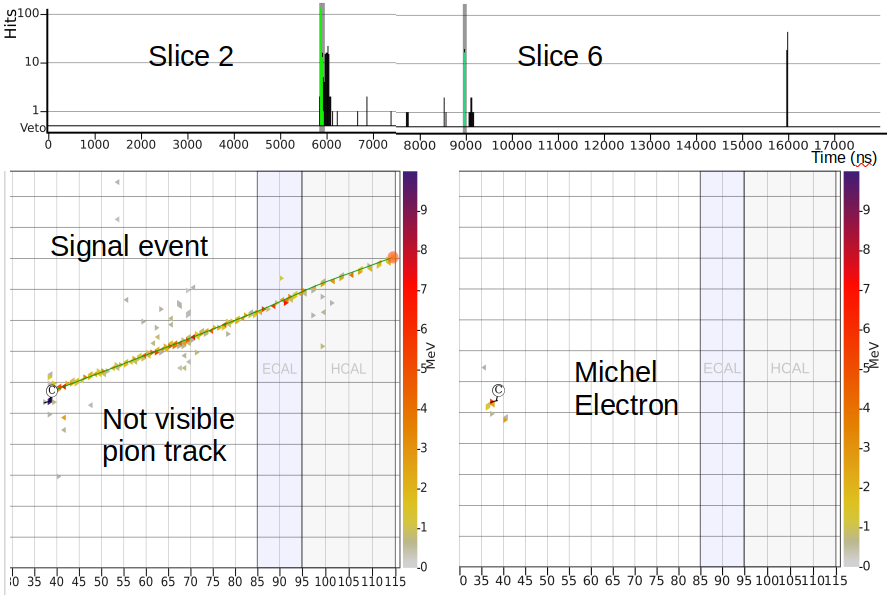
\includegraphics[scale=0.4]{Figures/Chapter4/DataSelection/EvenDisplayUntrackedSignalEventRun110000SubRun19Gate532.png}
    \caption{Event display of a MC event for an untracked pion for the the run 110000, subrun 19, Gate 532 for the XZ view. This figure shows and simulated signal event for the time slice 2 (left) and the time slice 6 (right). This shows an event where the michel electron is found. }
    \label{fig:Analysis:DataSelection:Cuts:Tracked:EventDisplayMEUntracked}
\end{figure}

The untracked event data selection gives an efficiency similar to that of tracked data selection. It is around 7\% and has a purity of 62\%. In the \textbf{Table} \ref{tab:Analysis:Cuts:UntrackedCutTable1} and \ref{tab:Analysis:Cuts:UntrackedCutTable2} the cut tables are shown for the untracked events. 

\begin{table}[!hbt]
    \tiny
    \centering
    \begin{tabular}{|*{7}{l|}}


    \hline
    & \multicolumn{4}{c|}{Signal} & \multicolumn{2}{c|}{Background} \\
    \hline
& N     & Eff     & Cut Eff & Pur    & N         & Eff   \\\hline
 No Cuts   & 203952.17     & 100.00\% & 100.00\% &   1.12\% & 17978780.42 & 100.00\% \\ \hline
 Anatool Precuts   & 159558.28     &  78.23\% &  78.23\% &   5.62\% & 2677126.18 &  14.89\% \\ \hline
 vertex position Cut   & 156840.33     &  76.90\% &  98.30\% &   5.79\% & 2551834.64 &  14.19\% \\ \hline
 MINOS Muon   & 151236.27     &  74.15\% &  96.43\% &   9.77\% & 1396389.62 &   7.77\%  \\ \hline
 1.5 GeV $<$ Pmu $<$ 20 GeV   & 150525.85     &  73.80\% &  99.53\% &  10.12\% & 1336621.79 &   7.43\%  \\ \hline
 $\theta_{\mu}$ $<$ 20 degrees   & 150457.23     &  73.77\% &  99.95\% &  10.30\% & 1310983.53 &   7.29\%  \\ \hline
 $<$2 Isolated Prongs   & 134544.17     &  65.97\% &  89.42\% &  17.94\% & 615463.26 &   3.42\%  \\ \hline
 Untracked Has Michel   & 61589.97     &  30.20\% &  45.78\% &  26.57\% & 170212.12 &   0.95\% \\ \hline
 Best Michel Distance   & 39690.52     &  19.46\% &  64.44\% &  43.88\% & 50759.18 &   0.28\% \\ \hline
 Closest Michel   & 39510.24     &  19.37\% &  99.55\% &  44.69\% & 48889.80 &   0.27\% \\ \hline
 One michel   & 14772.73     &   7.24\% &  37.39\% &  48.88\% & 15450.34 &   0.09\%  \\ \hline
 $T_\pi<$ 350 MeV   & 14766.17     &   7.24\% &  99.96\% &  49.42\% & 15111.12 &   0.08\% \\ \hline
 $Untracked W_{exp}$   & 14415.76     &   7.07\% &  97.63\% &  62.21\% & 8757.88 &   0.05\%  \\ \hline
    \end{tabular}
    \caption{P4 Cut Table, Untracked data selection (Part 1),\today. DataPOT: 89785235631482617856.00. MCPOT: 406599660544667287552.00..}
    \label{tab:Analysis:Cuts:UntrackedCutTable1}
\end{table}

\begin{table}[!hbt]
    \tiny
    \centering
    \begin{tabular}{|*{6}{l|}}


    \hline
    & \multicolumn{2}{c|}{Total} & \multicolumn{3}{c|}{Data} \\
    \hline
&  N         & Eff     & N MC (scale) & N Data    & Data/MC \\\hline
 No Cuts    & 18182732.59 & 100.00\% & NA & NA & NA \\ \hline
 Anatool Precuts  & 2836684.46 &  15.60\% & NA & NA & NA \\ \hline
 vertex position Cut  & 2708674.97     &  14.90\% & 598128.93     & 676952.00 &   1.13 \\ \hline
 MINOS Muon  & 1547625.89     &   8.51\% & 341746.36     & 358090.00 &   1.05 \\ \hline
 1.5 GeV $<$ Pmu $<$ 20 GeV   & 1487147.65     &   8.18\% & 328391.57     & 342163.00 &   1.04 \\ \hline
 $\theta_{\mu}$ $<$ 20 degrees   & 1461440.76     &   8.04\% & 322714.99     & 335784.00 &   1.04 \\ \hline
 $<$2 Isolated Prongs   & 750007.43     &   4.12\% & 165616.45     & 173567.00 &   1.05 \\ \hline
 Untracked Has Michel   & 231802.09     &   1.27\% & 51186.48     & 52895.00 &   1.03 \\ \hline
 Best Michel Distance   & 90449.70     &   0.50\% & 19973.08     & 20120.00 &   1.01 \\ \hline
 Closest Michel   & 88400.04     &   0.49\% & 19520.47     & 19759.00 &   1.01 \\ \hline
 One michel   & 30223.08     &   0.17\% & 6673.85     & 6874.00 &   1.03 \\ \hline
 $T_\pi<$ 350 MeV   & 29877.29     &   0.16\% & 6597.50     & 6826.00 &   1.03 \\ \hline
 $Untracked W_{exp}$  & 23173.64     &   0.13\% & 5117.20     & 5150.00 &   1.01 \\ \hline
    \end{tabular}
    \caption{P4 Cut Table, Untracked data selection (Part 2),\today. DataPOT: 89785235631482617856.00. MCPOT: 406599660544667287552.00..}
    \label{tab:Analysis:Cuts:UntrackedCutTable2}
\end{table}

\subsection{Special cut}
\label{Cap:Analysis:DataSelection:Cuts:SpecialCut}
According to the results presented in \ref{fig:Analysis:SignalDefinition:1DAnalysis:thetapivsTpi}, a special cut is made to the when measured $\theta_\pi$. The cut consists of only taking untracked pions with 20 MeV $< T_\pi < $ 350 MeV. The \textbf{Table} \textcolor{red}{Agregar la tabla para $\theta_\pi$} shows the results after to apply this cut to the sample.


\pagebreak

\subsubsection{Data selection combination}

The interest results from these analyses come to the fusion of the data selections described above, when these two data selections are combined to achieve the efficiency from \(\sim\) 6\% to \(\sim\) 12\% and the purity of 64\%. This combination also provides the opportunity to study a $T_\pi$ region that was not previously explored. 

When the two data selections are combined, the events that pass the cuts fall into one of three categories, \textit{Tracked Event}, \textit{Untracked Event} or \textit{Mixed Event}.
\begin{itemize}
    \item \textbf{Tracked Event}: it corresponds to an event that passes the tracked pion cuts but it fails the untracked pion cuts. In a tracked event, the central values of $T_\pi$ and $\theta_\pi$ are obtained using the information from the reconstructed pion track. For variables dependent on $E_{had}$ such as $W_{exp}$, $E_\nu$ and $Q^2$, $E_{had}$ is obtained by the \textbf{Equation} \ref{eq:EhadTracked}.
    \item \textbf{Untracked Event:} it corresponds to an event that passes the untracked pion cuts but it fails the tracked pion cuts. In a tracked event, the central values of $T_\pi$ and $\theta_\pi$ are obtained using the information of the michel electron. The reconstruction of these quantities is explained in \ref{Cap:MnvExp:MnvDetector:DataReconstruction:Untrackedpions}. For variables dependent on $E_{had}$ such as $W_{exp}$, $E_\nu$ and $Q^2$, $E_{had}$ is obtained by the \textbf{Equation} \ref{eq:EhadUntracked}.
    \item  \textbf{Mixed Event:} it corresponds to an event that passes tracked and untracked pion cuts. When an event falls into this category, the central value of all variables is obtained in the same way as a tracked event. 
\end{itemize}
The selection of the category is also explained in the flowchart of the \textbf{Figure} \ref{fig:Analysis:Cuts:Flowchart} 

\begin{figure}[!htb]
    \centering
    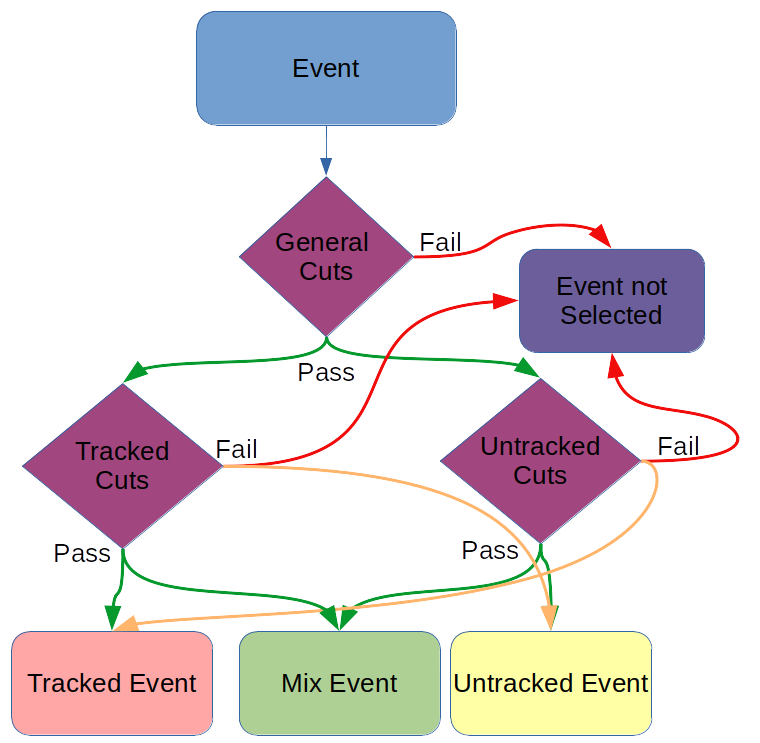
\includegraphics[scale=0.4]{Figures/Chapter4/DataSelection/EventSelFlowchart.png}
    \caption{Flowchart of of data selection for events when the tracked and untracked pions are included.}
    \label{fig:Analysis:Cuts:Flowchart}
\end{figure}

In the plot of the \textbf{Figure} \ref{fig:Analysis:Cuts:DataSelBreakdown}, this plot shows the different data selection components. It is observed that for low-$T_\pi$ region the most representative category is the untracked events, as is expected. And in accordance with the increase $T_\pi$, the number of tracked events increases with respect to the untracked. The percentage per category is shown in the \textbf{Table} \ref{tab:Analysis:Cuts:CategoryPercentage}.

\begin{figure}
    \centering
    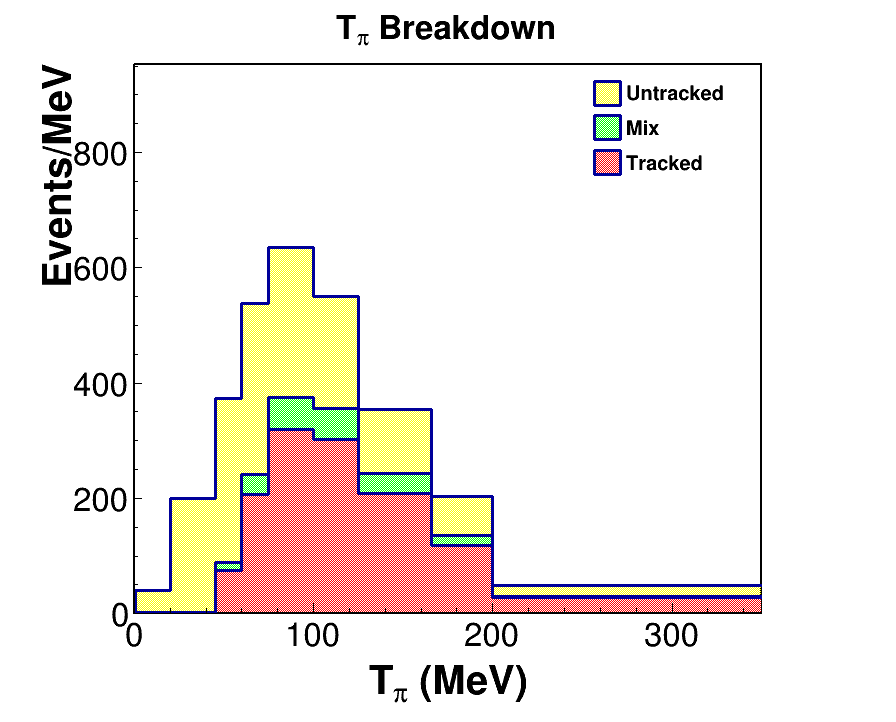
\includegraphics[scale=0.35]{Figures/Chapter4/DataSelection/Stacked_Tpi.png}
    \caption{Breakdown of data selection plot for the $T_\pi$ variable. The explains the category of the events.}
    \label{fig:Analysis:Cuts:DataSelBreakdown}
\end{figure}

\begin{table}[!htb]
    \centering
    \begin{tabular}{c|c}
         Category  & Percentage (\%) \\ \hline
         Tracked   &  40.3 \\
         Untracked &  47.6\\
         Mix       & 12.1
    \end{tabular}
    \caption{Percentage of events per category.}
    \label{tab:Analysis:Cuts:CategoryPercentage}
\end{table}

\subsection{Data Selection 1D analysis Results}
\label{Cap:Analysis:DataSelectionResults1D}

The results shown here were obtained using the MINER$\nu$A data for the whole data set of the ME era, with the beam in the neutrino mode. The data POT is 1.0$\times 10^{21}$. For MC, is used GENIE v2.12.6, with the MINER$\nu$A tunes MnvGENIEv4.3.1+ Pion Reweight.The POT for MC is 4.90$\times 10^{21}$.



%\foreach \var in {loW,midW,hiW}{ 
\foreach \var in  {enu,mixtpi,mixthetapi_deg,pmu,ptmu,pzmu,thetamu_deg,q2,wexp}{
%\foreach \var in  {enu_true,mixtpi_true,pmu_true,ptmu_true,pzmu_true,thetamu_deg_true,q2_true,wexp_true}{
    \ifthenelse{\equal{\var}{enu}}{
      \renewcommand{\NewVar}{E_\nu}
    }{}
    \ifthenelse{\equal{\var}{mixtpi}}{
      \renewcommand{\NewVar}{T_\pi}
    }{}
    \ifthenelse{\equal{\var}{mixthetapi_deg}}{
      \renewcommand{\NewVar}{\theta_\pi}
    }{}
    \ifthenelse{\equal{\var}{pmu}}{
      \renewcommand{\NewVar}{P_\mu}
    }{}
    \ifthenelse{\equal{\var}{ptmu}}{
      \renewcommand{\NewVar}{P^T_\mu}
    }{}
    \ifthenelse{\equal{\var}{pzmu}}{
      \renewcommand{\NewVar}{P^z_\mu}
    }{}
    \ifthenelse{\equal{\var}{thetamu_deg}}{
      \renewcommand{\NewVar}{\theta_\mu}
    }{}
    \ifthenelse{\equal{\var}{q2}}{
      \renewcommand{\NewVar}{Q^2}
    }{}
    \ifthenelse{\equal{\var}{wexp}}{
      \renewcommand{\NewVar}{W_{exp}}
    }{}
    \begin{figure}
        \centering
        \includegraphics[scale=0.3]{Figures/Chapter4/DataSelection/Selection_\var__1Pi_untunedBG_BWN.png}
        \caption{$\NewVar$ 1D Data Selection.}
        \label{fig:Analysis:DataSelResults:\var}
    \end{figure}  
}

\subsection{Data Selection 2D analysis Results}
\label{Cap:Analysis:DataSelectionResults2D}

For the 2D analysis, it only contains the tracked events, therefore the cut tables that correspond to this data selections \ref{tab:Analysis:Cuts:TrackedCutTable1} and \ref{tab:Analysis:Cuts:TrackedCutTable2}. For this data selection is used for the same data set that is used for the 1D analysis. For the simulation, the same simulation was used as for the 1D analysis. For this analysis the MC simulation is tuned by MnvGENIEv4.3.1, the Pion Reweighter is not applied because the trackless pions are not included in the data selection. 

%\foreach \var in {loW,midW,hiW}{ 
\foreach \var in  {ptmu_vs_tpi,tpi_vs_ptmu,ptmu_vs_pzmu,pzmu_vs_ptmu,tpi_vs_pmu,pmu_vs_tpi,thetapi_deg_vs_tpi,tpi_vs_thetapi_deg,enu_vs_tpi,tpi_vs_enu}{
%\foreach \var in  {enu_true,mixtpi_true,pmu_true,ptmu_true,pzmu_true,thetamu_deg_true,q2_true,wexp_true}{

    \ifthenelse{\equal{\var}{pzmu_vs_ptmu}}{
      \renewcommand{\NewVar}{P^z_\mu,P^T\mu}
    }{}
    \ifthenelse{\equal{\var}{tpi_vs_thetapi_deg}}{
      \renewcommand{\NewVar}{T_\pi,\theta_\pi}
    }{}
    \ifthenelse{\equal{\var}{tpi_vs_pmu}}{
      \renewcommand{\NewVar}{T_\pi,P_\mu}
    }{}
    \ifthenelse{\equal{\var}{ptmu_vs_tpi}}{
      \renewcommand{\NewVar}{P^T_\mu, T_\pi}
    }{}
    \ifthenelse{\equal{\var}{ptmu_vs_pzmu}}{
      \renewcommand{\NewVar}{P^T\mu, P^z_\mu}
    }{}
    \ifthenelse{\equal{\var}{thetapi_deg_vs_tpi}}{
      \renewcommand{\NewVar}{\theta_\pi, T_\pi}
    }{}
    \ifthenelse{\equal{\var}{pmu_vs_tpi}}{
      \renewcommand{\NewVar}{P_\mu, T\pi}
    }{}
    \ifthenelse{\equal{\var}{tpi_vs_ptmu}}{
      \renewcommand{\NewVar}{T_\pi,P^T_\mu}
    }{}
    \ifthenelse{\equal{\var}{tpi_vs_eu}}{
      \renewcommand{\NewVar}{T_\pi,E_\nu}
    }{}
    \ifthenelse{\equal{\var}{enu_vs_tpi}}{
      \renewcommand{\NewVar}{E_\nu, T_\pi}
    }{}
 
    \begin{figure}
        \centering
        \includegraphics[scale=0.3]{Figures/Chapter4/DataSelection/2D_Sel_\var__untunedBG__BWN.png}
        \caption{$\NewVar$ 2D Data Selection.}
        \label{fig:Analysis:DataSelResults:\var}
    \end{figure}  
}

\pagebreak



%++++++++++++++++++++++++++++++++++++++
%     Background Sustraction
%++++++++++++++++++++++++++++++++++++++
\section{Background studies}
\label{Cap:Analysis:BgStudies}
After the data selection is performed, the next step is to subtract the simulated background from the data selection. Before subtracting the simulated background from the data, the background tuning is made as was explained in the introduction. For the 1D and 2D analyses the same sideband tuning process is used, but since the 1D analysis includes the trackless events and for this analysis has 2 different $W_{exp}$ definitions, the final background weights are different for the 1D and 2D analyses. 





\subsection{Background tuning}
\label{Cap:Analysis:BgStudies:SidebandTuning}
For this analysis the mainly two sources of background come from events where the truth $W_{exp} >$ 1.4 GeV of events where the $T_\pi > $ 350 GeV. Most of the events with $W_{exp} > 1.4 $ MeV correspond to DIS events and some resonant events. The plots in the \textbf{Figure} \ref{fig:Analysis:BgStudies:SidebandTunning:BGBreakdownTpiWexp} show the different components of the background. In particular, the background that comes from the $W_{exp}$ miss reconstruction. 

\begin{figure}[!htb]
    \centering
    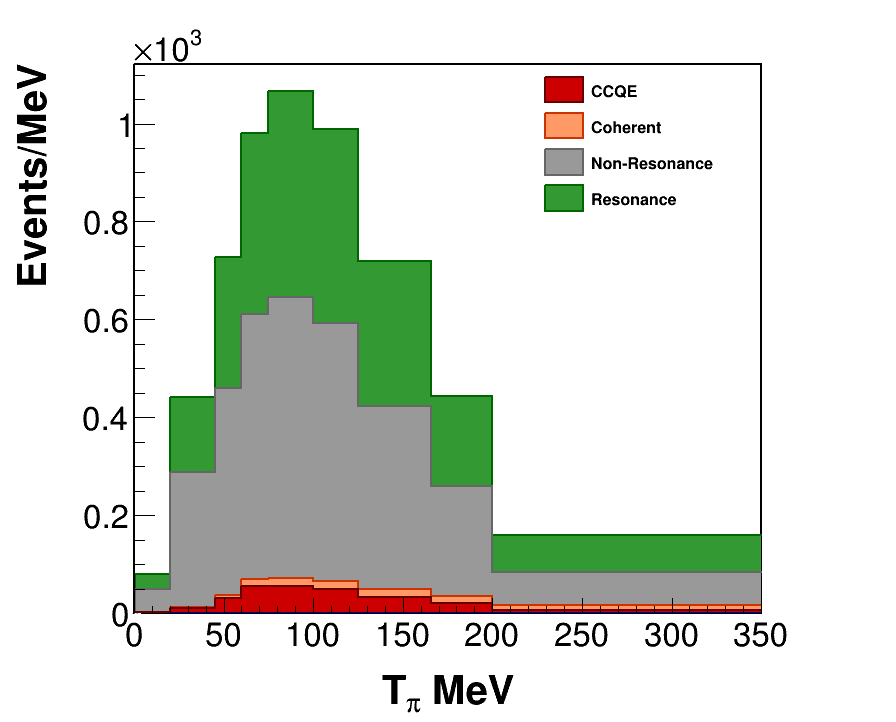
\includegraphics[scale=0.2]{Figures/Chapter4/BGStudies/Bd_Background_mixtpi_Int.png}
    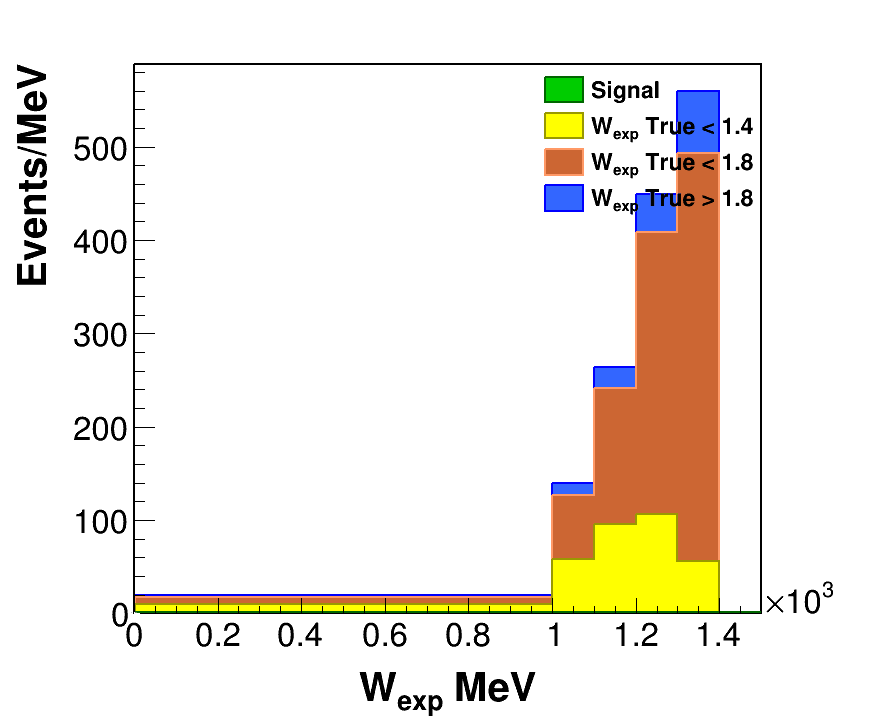
\includegraphics[scale=0.2]{Figures/Chapter4/BGStudies/Bd_Background_wexp_WSB.png}
    \caption{Breakdown background for $T_\pi$ (left) and $W_{exp}$ (right) variables. The left plot shows the different interactions types that make up the background of the data selection. The right plot shows the background components of the true $W_{exp}$.}
    \label{fig:Analysis:BgStudies:SidebandTunning:BGBreakdownTpiWexp}
\end{figure}

As mentioned in the Introduction, before to remove the simulated background, it is necessary to make a study to know how well the background is simulated. To make this study, a region that is not included by the signal definition but is kinematically adjacent is used. This region is known as the \textit{sideband}. Events are collected for data and MC, later the MC components of in the sideband region is scaled in situ to have a better agreement between data and MC in the sideband region. Later, the scale factor are applied to the components of MC but in the signal region, this procedure is known as the \textit{ background tuning}. This procedure helps to reduce the model dependency, reducing the systematic uncertainties. 

For these analyses, the sideband region is selected for all the events that pass the tracked and untracked pion cuts but with $W_{exp} > $ 1.5 GeV in the case of the 1D analysis and for the 2D analysis only the untracked pion events. The \textbf{Figure} \ref{fig:Analysis:BgStudies:SidebandTunning:BreakdownWSideband} shows the sideband region for the 1D analysis. 

\begin{figure}[!htb]
    \centering
    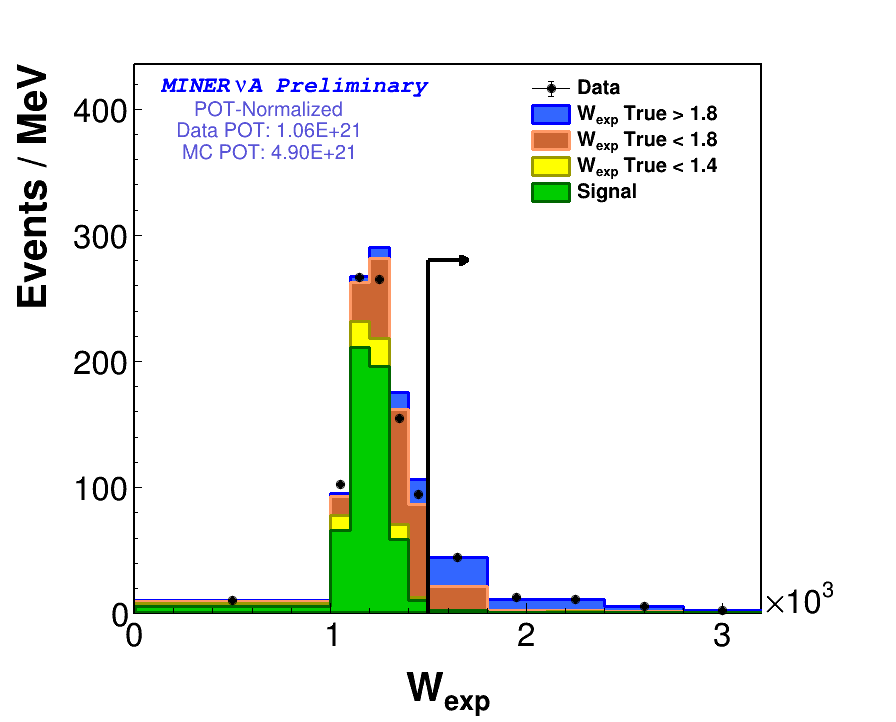
\includegraphics[scale=0.3]{Figures/Chapter4/BGStudies/Breakdown_WSideband_wexp_fit_1Pi_PN_.png}
    \caption{$W_{exp}$ breakdown histogram. This  shows the portion of events that are signal and background in all the $W_{exp}$ spectrum. The arrow shows the sideband region for the 1D analysis.}
    \label{fig:Analysis:BgStudies:SidebandTunning:BreakdownWSideband} 
\end{figure}

In the 1D analysis, if an event passes the tracked and untracked pion cuts prior to the $W_{exp}$ cut, the way to decide whether the event is a selected or sideband event and the central values that will be taken by the variables is shown in the \textbf{Table} \ref{tab:Analysis:BgStudies:SidebandTunning:WTruthTable}.


\begin{table}[!htb]
	
	\centering

	\begin{tabular}{c|c|c}
        Tracked           & Untracked         & Status \\ \hline
		\cellcolor{green} & \cellcolor{green} & \cellcolor{green} Tracked \\ \hline
		\cellcolor{green} & \cellcolor{orange} & \cellcolor{green} Tracked\\ \hline
  		\cellcolor{green} & \cellcolor{cyan} & \cellcolor{green} Tracked\\ \hline
		\cellcolor{orange} & \cellcolor{green} & \cellcolor{green} Untracked\\ \hline
  		\cellcolor{orange} & \cellcolor{orange} & \cellcolor{orange} Tracked\\ \hline
		\cellcolor{orange} & \cellcolor{cyan} & \cellcolor{cyan} Untracked\\ \hline
  		\cellcolor{cyan} & \cellcolor{green} & \cellcolor{green} Untracked\\ \hline
		\cellcolor{cyan} & \cellcolor{orange} & \cellcolor{cyan} Tracked\\ \hline
  		\cellcolor{cyan} & \cellcolor{cyan} & \cellcolor{cyan} Tracked\\ \hline
	\end{tabular}

    \caption{Truth table used to decide the status of an event passes the tracked and untracked previous cuts to the $W_{exp}$ is a selected event or sideband event, and if it is taking the values tracked or untracked central values. The colors code for the $W_{exp}$ regions are: \textbf{\textcolor{green}{GREEN}} color for $W_{exp}<$ 1.4 GeV, \textbf{\textcolor{orange}{ORANGE}} for 1.4 GeV $<W_{exp}<$ 1.5 GeV and \textbf{\textcolor{cyan}{ CYAN}} for $W_{exp}>$ 1.5 GeV. In the status column, it specify if the value for the event comes from the tracked or untracked $W_{exp}$ definition meanwhile the color \textbf{\textcolor{green}{GREEN}} is for for data selection events, \textbf{\textcolor{cyan}{CYAN}} for sideband and \textbf{\textcolor{orange}{ORANGE}} is not considered for either.}
	\label{tab:Analysis:BgStudies:SidebandTunning:WTruthTable}
\end{table}

For the cases where the event only passes tracked or untracked pion cuts, it just takes the central value of their respective type. For the 2D analysis, it is not necessary to use this table because it only use tracked pion events. 

The background is constrained by a iterative $\chi^2$ minimization technique:
\begin{equation}
    \chi^2=\sum^{N\ bins}_i \frac{\left(N_{simulation,i}-N_{Data,i}\right)^2}{\sigma^2_{simulation,i}+\sigma^2_{Data,i}},
\end{equation}

Where $N_{simulation}=N_{bakground}+N_{signal}$ in the sideband region and $N_{Data}$ is the data point in the simulated region. $N_{background}$  can be separated into components and scaled to fit the simulated distribution to the data distribution.  

In both analyses, the background events of the sideband region are separated into three components depending on their value $W_{exp}\ true$. The components are \textit{low} for $W_{exp}\ true<$ 1.4 GeV, \textit{ medium} for 1.4 GeV $<W_{exp}\ true< $ 1.8 GeV and \textit{high} for $W_{exp}\ true > 1.8$ GeV. The low upper limit is given because these are events that should be in the data selection region bet the $W_{exp}$ is not well reconstructed. The limit imposed between middle and high at 1.8 GeV is related to the simulation models, for $W < 1.8$ GeV the events are models by KNO + PYTHIA which includes resonant and hadronization production. For $W_{exp} > 1.8$ GeV the events are only modeled by PYTHIA, as explained in \ref{Cap:Simulation:GENIE}. The scale factors for the 1D and 2D analyses are shown in the \textbf{Table} \ref{tab:BgStudies:SidebandTunning:BGtunes}.

\begin{table}[!htb]
    \centering
    \begin{tabular}{c|c|c|c|c}
         Analysis & Low & Middle   &   High  & $\chi^2/ndf$ \\ \hline
         1D       & 1   & 0.969344 & 1.02864 & 2.37278 \\
         1D $\theta_\pi$& 1 & & & \\
         2D  & 1 &  0.715958 & 1.01369  & 1.80766
    \end{tabular}
    \caption{Results of the $\chi^2$ minimization to obtain the background tunes by components.}
    \label{tab:BgStudies:SidebandTunning:BGtunes}
\end{table}

In the \textbf{Figures} \ref{fig:Analysis:BgSub:enu}-\ref{fig:Analysis:BgSub:wexp} for the 1D, 1D $\theta_\pi$ signal and 2D analyses, respectively, the sideband region before and after the background fit is shown. 

\begin{figure}
    \centering
    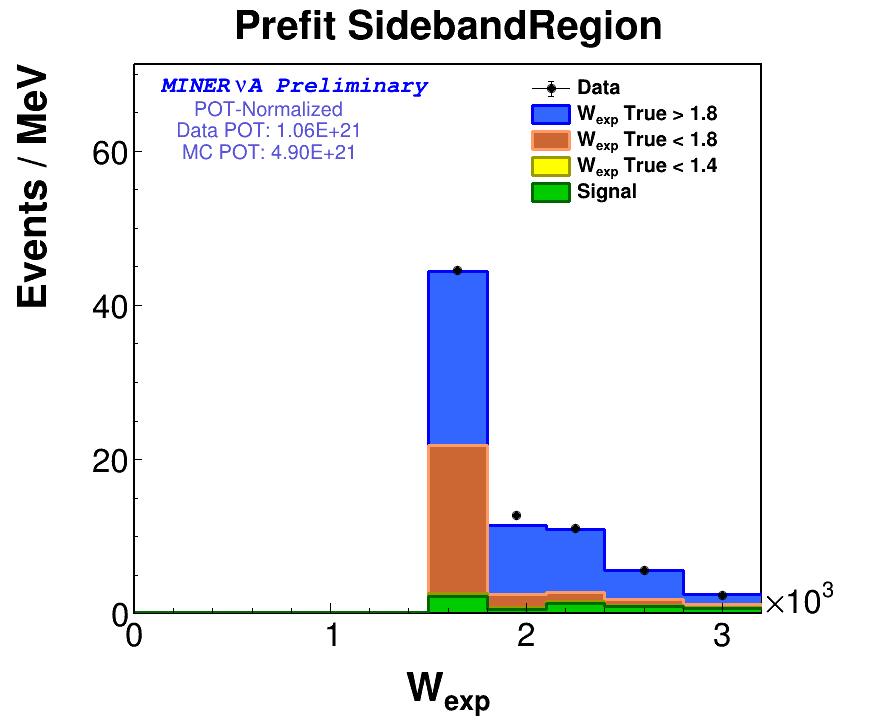
\includegraphics[scale=0.2]{Figures/Chapter4/BGStudies/PreWFit_wexp_fit_1Pi_PN_SidebandRegion_1DAnalysis.png}
    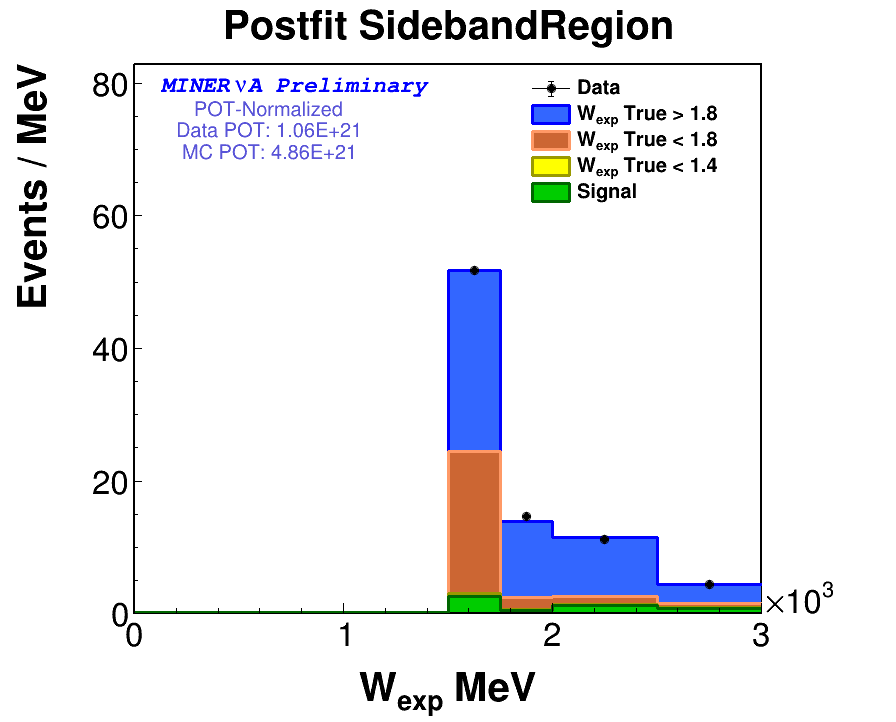
\includegraphics[scale=0.2]{Figures/Chapter4/BGStudies/PostWFit_wexp_fit_1Pi_PN_SidebandRegion_1DAnalysis.png}
    \caption{Pre-fitted (left) and post=fitted (right) MC sideband histograms for the 1D analysis.}
    \label{fig:BgStudies:SidebandTunning:PrePosFit1DAnalysis}
\end{figure}


\subsection{Background subtraction}
The following results correspond to the subtraction of the background of the 1D analysis. 

%\foreach \var in {loW,midW,hiW}{ 
\foreach \var in  {enu,mixtpi,mixthetapi_deg,pmu,ptmu,pzmu,thetamu_deg,q2,wexp}{
%\foreach \var in  {enu_true,mixtpi_true,pmu_true,ptmu_true,pzmu_true,thetamu_deg_true,q2_true,wexp_true}{
    \ifthenelse{\equal{\var}{enu}}{
      \renewcommand{\NewVar}{E_\nu}
    }{}
    \ifthenelse{\equal{\var}{mixtpi}}{
      \renewcommand{\NewVar}{T_\pi}
    }{}
    \ifthenelse{\equal{\var}{mixthetapi_deg}}{
      \renewcommand{\NewVar}{\theta_\pi}
    }{}
    \ifthenelse{\equal{\var}{pmu}}{
      \renewcommand{\NewVar}{P_\mu}
    }{}
    \ifthenelse{\equal{\var}{ptmu}}{
      \renewcommand{\NewVar}{P^T_\mu}
    }{}
    \ifthenelse{\equal{\var}{pzmu}}{
      \renewcommand{\NewVar}{P^z_\mu}
    }{}
    \ifthenelse{\equal{\var}{thetamu_deg}}{
      \renewcommand{\NewVar}{\theta_\mu}
    }{}
    \ifthenelse{\equal{\var}{q2}}{
      \renewcommand{\NewVar}{Q^2}
    }{}
    \ifthenelse{\equal{\var}{wexp}}{
      \renewcommand{\NewVar}{W_{exp}}
    }{}
    \begin{figure}
        \centering
        \includegraphics[scale=0.3]{Figures/Chapter4/BGStudies/BGSubData_\var__1Pi_BWN.png}
        \caption{$\NewVar$ 1D Background subtraction.}
        \label{fig:Analysis:BgSub:\var}
    \end{figure}  
}

%\foreach \var in {loW,midW,hiW}{ 
\foreach \var in  {ptmu_vs_tpi,tpi_vs_ptmu,ptmu_vs_pzmu,pzmu_vs_ptmu,tpi_vs_pmu,pmu_vs_tpi,thetapi_deg_vs_tpi,tpi_vs_thetapi_deg,enu_vs_tpi,tpi_vs_enu}{
%\foreach \var in  {enu_true,mixtpi_true,pmu_true,ptmu_true,pzmu_true,thetamu_deg_true,q2_true,wexp_true}{

    \ifthenelse{\equal{\var}{pzmu_vs_ptmu}}{
      \renewcommand{\NewVar}{P^z_\mu,P^T\mu}
    }{}
    \ifthenelse{\equal{\var}{tpi_vs_thetapi_deg}}{
      \renewcommand{\NewVar}{T_\pi,\theta_\pi}
    }{}
    \ifthenelse{\equal{\var}{tpi_vs_pmu}}{
      \renewcommand{\NewVar}{T_\pi,P_\mu}
    }{}
    \ifthenelse{\equal{\var}{ptmu_vs_tpi}}{
      \renewcommand{\NewVar}{P^T_\mu, T_\pi}
    }{}
    \ifthenelse{\equal{\var}{ptmu_vs_pzmu}}{
      \renewcommand{\NewVar}{P^T\mu, P^z_\mu}
    }{}
    \ifthenelse{\equal{\var}{thetapi_deg_vs_tpi}}{
      \renewcommand{\NewVar}{\theta_\pi, T_\pi}
    }{}
    \ifthenelse{\equal{\var}{pmu_vs_tpi}}{
      \renewcommand{\NewVar}{P_\mu, T\pi}
    }{}
    \ifthenelse{\equal{\var}{tpi_vs_ptmu}}{
      \renewcommand{\NewVar}{T_\pi,P^T_\mu}
    }{}
    \ifthenelse{\equal{\var}{tpi_vs_enu}}{
      \renewcommand{\NewVar}{T_\pi,E_\nu}
    }{}
    \ifthenelse{\equal{\var}{enu_vs_tpi}}{
      \renewcommand{\NewVar}{E_\nu, T_\pi}
    }{}
    \begin{figure}
        \centering
        \includegraphics[scale=0.3]{Figures/Chapter4/BGStudies/2D_BG_\var__BWN.png}
        \caption{$\NewVar$ 2D Background subtraction.}
        \label{fig:Analysis:BGSubtraction:\var}
    \end{figure}  
}

%++++++++++++++++++++++++++++++++++++++
%     Ungolding
%++++++++++++++++++++++++++++++++++++++

\section{Unfolding}
\label{Cap:Analysis:Unfolding}
As explained in the Introduction of the chapter, the unfolding process has the goal of removing the smearing effects in the distributions generated by detector deficiencies, detector resolution, detector geometry, etc. All these effects are simulated as well, as is possible to then apply these effects to the simulation to have a better comparison between the simulation data selection and data selection results. This can be represented as follow: 
\begin{equation}
    y_j=\sum^{truth\ bins}_i U_{ij}\lambda_i
    \label{eq:Analysis:unfolding:SmearingEq}
\end{equation}

where $y_j$ is the number of events reconstructed without background of the variable $y$ in the bin $j$, $U_{ij}$ is the migration matrix and $\lambda_i$ is the number of events in the truth bin $i$.

The $j$ column of the migration matrix has the fraction of reconstructed events that falls in the $j$ truth value. For this, the reconstructed event must be a signal event, and the truth and reconstructed binning have to be equal. In this way, the migration matrix gives information about how the variable is smeared, in an ideal detector, the migration matrix is an identity matrix ($\mathbb{I}_{truth\ bins}$).

In the \textbf{Figures} \ref{fig:Analysis:1DMigrationMtx:enu}-\ref{fig:Analysis:1DMigrationMtx:wexp} including the migration matrix $\theta_\pi$. The migration matrices present an absolute binning; this means that the X and Y axis binning correspond to the bin number. The actual binning is presented in the description of each variable. 

\foreach \var in  {enu,mixtpi,mixthetapi_deg,pmu,ptmu,pzmu,thetamu_deg,q2,wexp}{
%\foreach \var in  {enu_true,mixtpi_true,pmu_true,ptmu_true,pzmu_true,thetamu_deg_true,q2_true,wexp_true}{
    \ifthenelse{\equal{\var}{enu}}{
      \renewcommand{\NewVar}{E_\nu}
      \renewcommand{\Binning}{[0, 1000, 3000, 4000, 6000, 9000, 14000, 30000] MeV}
    }{}
    \ifthenelse{\equal{\var}{mixtpi}}{
      \renewcommand{\NewVar}{T_\pi}
      \renewcommand{\Binning}{[0, 20, 45, 60, 75, 100, 125, 166, 200, 350] MeV}
    }{}
    \ifthenelse{\equal{\var}{mixthetapi_deg}}{
      \renewcommand{\NewVar}{\theta_\pi}
      \renewcommand{\Binning}{[0, 15, 30, 45, 60, 76, 108, 122, 136, 150, 165, 180] degrees}
    }{}
    \ifthenelse{\equal{\var}{pmu}}{
      \renewcommand{\NewVar}{P_\mu}
      \renewcommand{\Binning}{[0, 1000,  2000,  3000,  4000, 5000, 7000, 10000, 13000, 20000, 30000] MeV}
    }{}
    \ifthenelse{\equal{\var}{ptmu}}{
      \renewcommand{\NewVar}{P^T_\mu}
      \renewcommand{\Binning}{[0, 100, 200,  300,   400,  500, 600, 800, 1000, 1200, 1500, 2500] MeV}
    }{}
    \ifthenelse{\equal{\var}{pzmu}}{
      \renewcommand{\NewVar}{P^z_\mu}
      \renewcommand{\Binning}{[0, 1000, 2000,  3000,  4000, 5000, 6000, 8000, 10000, 15000, 20000] MeV}
    }{}
    \ifthenelse{\equal{\var}{thetamu_deg}}{
      \renewcommand{\NewVar}{\theta_\mu}
      \renewcommand{\Binning}{[0, 1, 2,  3,  4,  5,  6, 7, 8, 9, 10, 11, 12, 14 , 16 , 20] degree}
    }{}
    \ifthenelse{\equal{\var}{q2}}{
      \renewcommand{\NewVar}{Q^2}
      \renewcommand{\Binning}{[0, 0.025e6, 0.05e6, 0.1e6, 0.2e6, 0.3e6, 0.4e6, 0.5e6, 0.7e6, 1.0e6, 1.3e6, 2.0e6, 3.0e6] MeV\( ^2\)}
    }{}
    \ifthenelse{\equal{\var}{wexp}}{
      \renewcommand{\NewVar}{W_{exp}}
      \renewcommand{\Binning}{[0, 1000, 1100, 1200, 1300, 1400, 1500] MeV}
    }{}
    \begin{figure}[!htb]
        \centering
        \includegraphics[scale=0.28]{Figures/Chapter4/Unfolding/Migration_AbsBins_\var.png}
        \caption{$\NewVar$ 1D Migration Matrix. The binning for the variable is \Binning.}
        \label{fig:Analysis:1DMigrationMtx:\var}
    \end{figure}  
}
\pagebreak

For the 2D analysis, the smearing effects are observed with respect to two variables. For the 2D analysis the smearing is described by:
\begin{equation}
    d_{ij}=\sum^{n}_{a}\sum^{m}_{b}U_{abij}\rho_{ab},
    \label{eq:Analysis:unfolding:SmearingEq2D}
\end{equation}

where $d$ is the number of events reconstructed for the bins $i$ and $j$ for the variables $x$ and $y$, respectively. $rho$ is the number of events for the truth $a$ and $b$ bins for the variables $x$ and $y$, respectively. $n$ and $m$ are the number of bins for the variable $x$ and $y$, respectively. $U_{abij}$ is a migration matrix in four dimensions, similar to the 1D analysis migration matrix, it contains the information of the fraction of reconstructed events that fall in a true bin, in this case it is observed as a function of two variables. For obvious reasons, the four-dimensional matrix cannot be plotted, but the projections of the 2D migration matrix of the $x$ in the $y$ migration matrix can be used. These migration matrices for the 2D analysis are shown in the \textbf{Figures} \ref{fig:Analysis:2DMigrationMatrix:ptmu_vs_tpi}-\ref{fig:Analysis:2DMigrationMatrix:tpi_vs_enu}

%\foreach \var in {loW,midW,hiW}{ 
\foreach \var in  {ptmu_vs_tpi,tpi_vs_ptmu,ptmu_vs_pzmu,pzmu_vs_ptmu,tpi_vs_pmu,pmu_vs_tpi,thetapi_deg_vs_tpi,tpi_vs_thetapi_deg,enu_vs_tpi,tpi_vs_enu}{
%\foreach \var in  {enu_true,mixtpi_true,pmu_true,ptmu_true,pzmu_true,thetamu_deg_true,q2_true,wexp_true}{

    \ifthenelse{\equal{\var}{pzmu_vs_ptmu}}{
      \renewcommand{\NewVar}{P^z_\mu,P^T\mu}
      \renewcommand{\Binning}{[1500, 2500, 3750, 4750, 5250, 8250, 20000] MeV, [0, 150, 300, 400, 550, 650, 2000] MeV}
    }{}
    \ifthenelse{\equal{\var}{ptmu_vs_pzmu}}{
      \renewcommand{\NewVar}{P^T_\mu,P^z\mu}
      \renewcommand{\Binning}{[0, 150, 300, 400, 550, 650, 2000] MeV, [1500, 2500, 3750, 4750, 5250, 8250, 20000] MeV}
    }{}
    
    \ifthenelse{\equal{\var}{tpi_vs_thetapi_deg}}{
      \renewcommand{\NewVar}{T_\pi,\theta_\pi}
      \renewcommand{\Binning}{[35, 100, 150, 200, 350] MeV, [0, 15, 30, 45, 60, 76, 108, 136, 180] degree}
    }{}
    \ifthenelse{\equal{\var}{thetapi_deg_vs_tpi}}{
      \renewcommand{\NewVar}{\theta_\pi,T_\pi}
      \renewcommand{\Binning}{[0, 15, 30, 45, 60, 76, 108, 136, 180] degree, [35, 100, 150, 200, 350] MeV}
    }{}

    \ifthenelse{\equal{\var}{tpi_vs_pmu}}{
      \renewcommand{\NewVar}{T_\pi,P_\mu}
      \renewcommand{\Binning}{[35., 100., 150., 200., 350.] MeV, [1500, 3000, 4000, 5500, 7500, 10000, 13000, 20000] MeV}
    }{}
    \ifthenelse{\equal{\var}{pmu_vs_tpi}}{
      \renewcommand{\NewVar}{P_\mu,T_\pi}
      \renewcommand{\Binning}{[1500, 3000, 4000, 5500, 7500,
                10000, 13000, 20000] MeV, [35., 100., 150., 200., 350.] MeV}
    }{}

    \ifthenelse{\equal{\var}{ptmu_vs_tpi}}{
      \renewcommand{\NewVar}{P^T_\mu, T_\pi}
      \renewcommand{\Binning}{[0, 270, 420, 600, 800, 1100, 2000] MeV, [35, 100, 150, 200, 350] MeV}
    }{}
    \ifthenelse{\equal{\var}{tpi_vs_ptmu}}{
      \renewcommand{\NewVar}{T_\pi, P^T_\mu}
      \renewcommand{\Binning}{[35, 100, 150, 200, 350] MeV, [0, 270, 420, 600, 800, 1100, 2000] MeV}
    }{}
 
    \ifthenelse{\equal{\var}{enu_vs_tpi}}{
      \renewcommand{\NewVar}{E_\nu, T_\pi}
      \renewcommand{\Binning}{[0, 1000, 3000, 4000, 6500, 9500, 14000, 30000] MeV, [35, 100, 150, 200, 350] MeV}
    }{}
    \ifthenelse{\equal{\var}{tpi_vs_enu}}{
      \renewcommand{\NewVar}{T_\pi, E_\nu}
      \renewcommand{\Binning}{[35, 100, 150, 200, 350] MeV, [0, 1000, 3000, 4000, 6500, 9500, 14000, 30000] MeV}
    }{}
    \begin{figure}
        \centering
        \includegraphics[scale=0.3]{Figures/Chapter4/Unfolding/2D_Migration_VarBins_\var.png}
        \caption{$\NewVar$ 2D Migration matrix, with binning \Binning $\ $respectively. }
        \label{fig:Analysis:2DMigrationMatrix:\var}
    \end{figure}  
}





\pagebreak
\subsection{Warping Studies}
\label{Cap:Analysis:Unfolding:WarpingStudies}

At this point, the smeared model can be compared with the data, but usually one is interested to compare the results with not only one model or with the results of other experiments. Reason why the importance of the unfolding process. This process is the inverse process of what is shown in \ref{eq:Analysis:unfolding:SmearingEq} and \ref{eq:Analysis:unfolding:SmearingEq2D}, it means that given a reconstructed distribution to obtain the truth distribution. In this way, the data results can be compared with other models or other experiments. Unfortunately, most of the migration matrices are not analytically invertible matrices. Hence, the migration matrix is inverted by a numerical iterative method based on the D'Agostini method \cite{DAGOSTINI1995487}\cite{dagostini2010improved}. For this method, as the number of iterations increases, the variance decreases but at the cost of increasing bias, the increase of the bias can be moderated, truncating the number of iterations. To determine the number of iterations, the minimum number of necessary iterations to stabilize the bias to a minimum is used. The bias is given by:

\begin{equation}
    \chi^2 = \sum_{\alpha\beta}(\hat{\lambda}^{(k)}-\lambda)_\beta V^{-1}_{\beta\alpha} (\hat{\lambda}^{(k)}-\lambda)_\alpha,
    \label{eq:Analysis:Unfolding:chi2WarpingStudies}
\end{equation}

where $\lambda$ corresponds to the number of events in the true distribution, $\hat{\lambda}^{(k)}$ corresponds to the unfolded distribution after $k$ iterations, $\alpha$ and $\beta$ are the bins of the unfolded distribution and $V$ is the unfolding covariance matrix.  

The number of iterations used to unfold the reconstructed distribution is obtained by the \textit{Warping Study}. It consists of using a nominal distribution that will be used as the truth distribution and a reweighted distribution, or "warped" distribution. This is made with the aim of testing the unfold procedure with different models that determine the sensitivity by the different weights. The $\chi^2$  obtained in \ref{eq:Analysis:Unfolding:chi2WarpingStudies} is obtained for each iteration in N universes, in this analysis N=500. The universes are used to consider statistical fluctuations. The selected number of iterations corresponds to the minimum $\chi^2$ media.

This procedure is used for all the variables that are presented in the analysis. For this analysis, 3 different models were used to warp the nominal distributions. The models are as follows.

\begin{itemize}
    \item \textbf{Resonant $M^{RES}_A$ Warp (WARP1)}: The resonant axial mass in the Rein-Seghal model is shifted by +1 $\sigma$. In the \textbf{Chapter} \ref{Cap:Simulation:MnvGENIETunes} it is explained.
    \item \textbf{Anisotropic $\Delta$ Decay Warp (WARP2)}: This weight modifies the angular $\Delta$ angular distribution. In the \textbf{Chapter} \ref{Cap:Simulation:MnvGENIETunes} it is explained. 
    \item \textbf{MK Warp(WARP3)}: This weight modifies the single pion production events. The MK model \cite{MK:PhysRevD.97.013002} is an extension of the Rein-Seghal model.
\end{itemize}

These three warps were used for the 1D analysis and the 2D analysis. In the \textbf{Figures} \ref{fig:Analysis:Unfolding:1DWarpingStudiesenu}-\ref{fig:Analysis:Unfolding:1DWarpingStudieswexp} the results for the 1D and 2D analysis are shown. In the results, it shows the number of iterations as a function of the number of iterations. This shows a histogram of the value of $\chi^2$ for the 500 universes, the average $\chi^2$, the median, the truncated $\chi^2$ mean, and the number of degrees of freedom (ndf). The expected result is that the number and value of $\chi^2$ approach ndf. 

\foreach \var in  {enu,mixtpi,mixthetapi_deg,pmu,ptmu,pzmu,thetamu_deg,q2,wexp}{
%\foreach \var in  {enu_true,mixtpi_true,pmu_true,ptmu_true,pzmu_true,thetamu_deg_true,q2_true,wexp_true}{
    \ifthenelse{\equal{\var}{enu}}{
      \renewcommand{\NewVar}{E_\nu}
    }{}
    \ifthenelse{\equal{\var}{mixtpi}}{
      \renewcommand{\NewVar}{T_\pi}
    }{}
    \ifthenelse{\equal{\var}{mixthetapi_deg}}{
      \renewcommand{\NewVar}{\theta_\pi}
    }{}
    \ifthenelse{\equal{\var}{pmu}}{
      \renewcommand{\NewVar}{P_\mu}
    }{}
    \ifthenelse{\equal{\var}{ptmu}}{
      \renewcommand{\NewVar}{P^T_\mu}
    }{}
    \ifthenelse{\equal{\var}{pzmu}}{
      \renewcommand{\NewVar}{P^z_\mu}
    }{}
    \ifthenelse{\equal{\var}{thetamu_deg}}{
      \renewcommand{\NewVar}{\theta_\mu}
    }{}
    \ifthenelse{\equal{\var}{q2}}{
      \renewcommand{\NewVar}{Q^2}
    }{}
    \ifthenelse{\equal{\var}{wexp}}{
      \renewcommand{\NewVar}{W_{exp}}
    }{}
    \begin{figure}
        \centering
        \includegraphics[scale=0.3]{Figures/Chapter4/Unfolding/Warping_\var_WARP1.png}
        \includegraphics[scale=0.3]{Figures/Chapter4/Unfolding/Warping_\var_WARP2.png}
        \includegraphics[scale=0.3]{Figures/Chapter4/Unfolding/Warping_\var_WARP3.png}
        \caption{$\NewVar$ 1D Warping studies results.}
        \label{fig:Analysis:Unfolding:1DWarpingStudies\var}
    \end{figure}  
}

%\foreach \var in {loW,midW,hiW}{ 
\foreach \var in  {ptmu_vs_tpi,tpi_vs_ptmu,ptmu_vs_pzmu,pzmu_vs_ptmu,tpi_vs_pmu,pmu_vs_tpi,thetapi_deg_vs_tpi,tpi_vs_thetapi_deg,enu_vs_tpi,tpi_vs_enu}{
%\foreach \var in  {enu_true,mixtpi_true,pmu_true,ptmu_true,pzmu_true,thetamu_deg_true,q2_true,wexp_true}{

    \ifthenelse{\equal{\var}{pzmu_vs_ptmu}}{
      \renewcommand{\NewVar}{P^z_\mu,P^T\mu}
    }{}
    \ifthenelse{\equal{\var}{tpi_vs_thetapi_deg}}{
      \renewcommand{\NewVar}{T_\pi,\theta_\pi}
    }{}
    \ifthenelse{\equal{\var}{tpi_vs_pmu}}{
      \renewcommand{\NewVar}{T_\pi,P_\mu}
    }{}
    \ifthenelse{\equal{\var}{ptmu_vs_tpi}}{
      \renewcommand{\NewVar}{P^T_\mu, T_\pi}
    }{}
    \ifthenelse{\equal{\var}{ptmu_vs_pzmu}}{
      \renewcommand{\NewVar}{P^T\mu, P^z_\mu}
    }{}
    \ifthenelse{\equal{\var}{thetapi_deg_vs_tpi}}{
      \renewcommand{\NewVar}{\theta_\pi, T_\pi}
    }{}
    \ifthenelse{\equal{\var}{pmu_vs_tpi}}{
      \renewcommand{\NewVar}{P_\mu, T\pi}
    }{}
    \ifthenelse{\equal{\var}{tpi_vs_ptmu}}{
      \renewcommand{\NewVar}{T_\pi,P^T_\mu}
    }{}
    \ifthenelse{\equal{\var}{tpi_vs_enu}}{
      \renewcommand{\NewVar}{T_\pi,E_\nu}
    }{}
    \ifthenelse{\equal{\var}{enu_vs_tpi}}{
      \renewcommand{\NewVar}{E_\nu, T_\pi}
    }{}
    \begin{figure}
        \centering
        \includegraphics[scale=0.3]{Figures/Chapter4/Unfolding/Warping_20240117_\var_WARP1.png}
        \includegraphics[scale=0.3]{Figures/Chapter4/Unfolding/Warping_20240117_\var_WARP2.png}
        \includegraphics[scale=0.3]{Figures/Chapter4/Unfolding/Warping_20240117_\var_WARP3.png}
        \caption{$\NewVar$ 2D warping studies results}
        \label{fig:Analysis:Unfolding:2DWarping\var}
    \end{figure}  
}

There are some variables, such as $W_{exp}$ where the $\chi^2$ values never converge to the ndf, for these cases the number of iterations is fixed at 10. These variables are highly dependent on the model and cannot be successfully unfolded. Results obtained for these variables do not pass the required test and, therefore, cannot be published. However, they can be reported internally within the collaboration and in this thesis. The number of iterations that will be used for the 1D analysis and 2D analysis are shown in the \textbf{Tables} \ref{tab:Analysis:Unfolding:1DIterations} and \ref{tab:Analysis:Unfolding:2DIterations}.
\begin{table}[!htb]
    \centering
    \begin{tabular}{c|c}
        Variable & Number of iterations \\ \hline
        $E_\nu$  & 3\\
        $T_\pi$  & 4\\
        $\theta_\pi$ & 8\\
        $P_\mu$ & 3\\
        $P^T_\mu$ & 4\\
        $P^z_\mu$ & 3\\
        $\theta_\mu$ & 2 \\
        $Q^2$ & 8\\
        $W_{exp}$ & 10
    \end{tabular}
    \caption{The value is obtained by initially selecting the first \textbf{\# of iterations} bin that approaches the ndf. Subsequently, a comparison is made between the different warps, and the higher number among the warps is chosen.}
    \label{tab:Analysis:Unfolding:1DIterations}
\end{table}

\begin{table}[!htb]
    \centering
    \begin{tabular}{c|c}
        Variable & Number of iterations \\ \hline
        $P^T_\mu$ vs $T_\pi$ and $T_\pi$ vs $P^T_\mu$ & 5\\
        $P^T_\mu$ vs $P^z_\mu$ and $P^z_\mu$ vs $P^T_\mu$ & 4\\
        $P_\mu$ vs $T_\pi$ and $T_\pi$ vs $P_\mu$ & 5\\
        $\theta_\pi$ vs $T_\pi$ and $T_\pi$ vs $\theta_\pi$ & 10\\
        $E_\nu$ vs $T_\pi$ and $T_\pi$ vs $E_\nu$ & 8
    \end{tabular}
    \caption{The value is obtained by initially selecting the first \textbf{\# of iterations} bin that approaches the ndf. Subsequently, a comparison is made between the different warps, and the higher number among the warps is chosen.}
    \label{tab:Analysis:Unfolding:2DIterations}
\end{table}


\subsection{Unfolded Distributions}
\label{Cap:Analysis:Unfolding:nfoldingResults}
Using the number of iterations obtained from the warping studies, the unfolding for all the variables were obtained. The unfolding process move events for one bin to other, changing the statistical error between in the bins. This produces a correlation between the statistical error. It can be represented in a covariance matrix. At the same time the unfolding process is made to the systematic universes to get the error propagation in the whole cross section measurement. The results of the unfolding are shown in the \textbf{Figures} \ref{fig:Analysis:Unfolding:1DUnfoldedenu}-\ref{fig:Analysis:Unfolding:1DUnfoldedwexp} for the 1D analysis and \ref{fig:Analysis:Unfolding:2DUnfoldedptmu_vs_tpi}-\ref{fig:Analysis:Unfolding:2DUnfoldedtpi_vs_enu} for the 2D analysis.

\foreach \var in  {enu,mixtpi,mixthetapi_deg,pmu,ptmu,pzmu,thetamu_deg,q2,wexp}{
%\foreach \var in  {enu_true,mixtpi_true,pmu_true,ptmu_true,pzmu_true,thetamu_deg_true,q2_true,wexp_true}{
    \ifthenelse{\equal{\var}{enu}}{
      \renewcommand{\NewVar}{E_\nu}
    }{}
    \ifthenelse{\equal{\var}{mixtpi}}{
      \renewcommand{\NewVar}{T_\pi}
    }{}
    \ifthenelse{\equal{\var}{mixthetapi_deg}}{
      \renewcommand{\NewVar}{\theta_\pi}
    }{}
    \ifthenelse{\equal{\var}{pmu}}{
      \renewcommand{\NewVar}{P_\mu}
    }{}
    \ifthenelse{\equal{\var}{ptmu}}{
      \renewcommand{\NewVar}{P^T_\mu}
    }{}
    \ifthenelse{\equal{\var}{pzmu}}{
      \renewcommand{\NewVar}{P^z_\mu}
    }{}
    \ifthenelse{\equal{\var}{thetamu_deg}}{
      \renewcommand{\NewVar}{\theta_\mu}
    }{}
    \ifthenelse{\equal{\var}{q2}}{
      \renewcommand{\NewVar}{Q^2}
    }{}
    \ifthenelse{\equal{\var}{wexp}}{
      \renewcommand{\NewVar}{W_{exp}}
    }{}
    \begin{figure}
        \centering
        \includegraphics[scale=0.3]{Figures/Chapter4/Unfolding/Unfolded_\var__1Pi_BWN.png}
        \caption{$\NewVar$ 1D Unfolded histogram.}
        \label{fig:Analysis:Unfolding:1DUnfolded\var}
    \end{figure}  
}

%\foreach \var in {loW,midW,hiW}{ 
\foreach \var in  {ptmu_vs_tpi,tpi_vs_ptmu,ptmu_vs_pzmu,pzmu_vs_ptmu,tpi_vs_pmu,pmu_vs_tpi,thetapi_deg_vs_tpi,tpi_vs_thetapi_deg,enu_vs_tpi,tpi_vs_enu}{
%\foreach \var in  {enu_true,mixtpi_true,pmu_true,ptmu_true,pzmu_true,thetamu_deg_true,q2_true,wexp_true}{

    \ifthenelse{\equal{\var}{pzmu_vs_ptmu}}{
      \renewcommand{\NewVar}{P^z_\mu,P^T\mu}
    }{}
    \ifthenelse{\equal{\var}{tpi_vs_thetapi_deg}}{
      \renewcommand{\NewVar}{T_\pi,\theta_\pi}
    }{}
    \ifthenelse{\equal{\var}{tpi_vs_pmu}}{
      \renewcommand{\NewVar}{T_\pi,P_\mu}
    }{}
    \ifthenelse{\equal{\var}{ptmu_vs_tpi}}{
      \renewcommand{\NewVar}{P^T_\mu, T_\pi}
    }{}
    \ifthenelse{\equal{\var}{ptmu_vs_pzmu}}{
      \renewcommand{\NewVar}{P^T\mu, P^z_\mu}
    }{}
    \ifthenelse{\equal{\var}{thetapi_deg_vs_tpi}}{
      \renewcommand{\NewVar}{\theta_\pi, T_\pi}
    }{}
    \ifthenelse{\equal{\var}{pmu_vs_tpi}}{
      \renewcommand{\NewVar}{P_\mu, T\pi}
    }{}
    \ifthenelse{\equal{\var}{tpi_vs_ptmu}}{
      \renewcommand{\NewVar}{T_\pi,P^T_\mu}
    }{}
    \ifthenelse{\equal{\var}{tpi_vs_enu}}{
      \renewcommand{\NewVar}{T_\pi,E_\nu}
    }{}
    \ifthenelse{\equal{\var}{enu_vs_tpi}}{
      \renewcommand{\NewVar}{E_\nu, T_\pi}
    }{}
    \begin{figure}
        \centering
        \includegraphics[scale=0.3]{Figures/Chapter4/Unfolding/2D_Unfolded_\var__BWN.png}
        \caption{$\NewVar$ 2D Unfolded histogram}
        \label{fig:Analysis:Unfolding:2DUnfolded\var}
    \end{figure}  
}

\pagebreak
%++++++++++++++++++++++++++++++++++++++
%     Efficiency  
%++++++++++++++++++++++++++++++++++++++

\section{Efficiency correction}
\label{Cap:Analysis:Efficiency}

In the introduction of the chapter the efficiency correction and the efficiency definition in the \textbf{Equation} \ref{eq:Analysis:efficiency} are described. The efficiency correction consists of dividing the unfolded distribution by the efficiency of each bin. It can be described as follows for the 1D analysis:

\begin{equation}
    N_i = \frac{\lambda_i}{\epsilon_i}
    \label{eq:Analysis:Efficiency:1DEfficiencyCorrection}
\end{equation}

where $N_i$ is the number of signal events in the bin $i$, $\lambda_i$ is the unfolded events in the bin $i$ and $\epsilon_i$ is the efficiency value of the bin $i$. In the case of the 2D analysis, we obtain the following relation: 

\begin{equation}
    N_{ij} = \frac{\rho_{ij}}{\epsilon_{ij}}
    \label{eq:Analysis:Efficiency:2DEfficiencyCorrection}
\end{equation}

where $N_{ij}$ is the number of signal events in the bin $i,j$, $\rho_i$ is the unfolded events in the bin $i,j$ and $\epsilon_{ij}$ is the efficiency value of the bin $i,j$.
In the \textbf{Figures} \ref{fig:Analysis:Unfolding:1DEfficiencyenu}-\ref{fig:Analysis:Unfolding:1DEfficiencywexp} and \ref{fig:Analysis:Unfolding:2DEfficiencyptmu_true_vs_tpi_true}-\ref{fig:Analysis:Unfolding:2DEfficiencytpi_true_vs_enu_true} the efficiency histograms for the 1D and 2D analysis, respectively, are shown. 
\subsection{Efficiency histograms}
\foreach \var in  {enu,mixtpi,mixthetapi_deg,pmu,ptmu,pzmu,thetamu_deg,q2,wexp}{
%\foreach \var in  {enu_true,mixtpi_true,pmu_true,ptmu_true,pzmu_true,thetamu_deg_true,q2_true,wexp_true}{
    \ifthenelse{\equal{\var}{enu}}{
      \renewcommand{\NewVar}{E_\nu}
    }{}
    \ifthenelse{\equal{\var}{mixtpi}}{
      \renewcommand{\NewVar}{T_\pi}
    }{}
    \ifthenelse{\equal{\var}{mixthetapi_deg}}{
      \renewcommand{\NewVar}{\theta_\pi}
    }{}
    \ifthenelse{\equal{\var}{pmu}}{
      \renewcommand{\NewVar}{P_\mu}
    }{}
    \ifthenelse{\equal{\var}{ptmu}}{
      \renewcommand{\NewVar}{P^T_\mu}
    }{}
    \ifthenelse{\equal{\var}{pzmu}}{
      \renewcommand{\NewVar}{P^z_\mu}
    }{}
    \ifthenelse{\equal{\var}{thetamu_deg}}{
      \renewcommand{\NewVar}{\theta_\mu}
    }{}
    \ifthenelse{\equal{\var}{q2}}{
      \renewcommand{\NewVar}{Q^2}
    }{}
    \ifthenelse{\equal{\var}{wexp}}{
      \renewcommand{\NewVar}{W_{exp}}
    }{}
    \begin{figure}
        \centering
        \includegraphics[scale=0.3]{Figures/Chapter4/Efficiency/Efficiency_\var_true.png}
        \caption{$\NewVar$ 1D Efficiency histogram.}
        \label{fig:Analysis:Unfolding:1DEfficiency\var}
    \end{figure}  
}

%\foreach \var in {loW,midW,hiW}{ 
\foreach \var in  {ptmu_true_vs_tpi_true,tpi_true_vs_ptmu_true,ptmu_true_vs_pzmu_true,pzmu_true_vs_ptmu_true,tpi_true_vs_pmu_true,pmu_true_vs_tpi_true,thetapi_deg_true_vs_tpi_true,tpi_true_vs_thetapi_deg_true,enu_true_vs_tpi_true,tpi_true_vs_enu_true}{
%\foreach \var in  {enu_true,mixtpi_true,pmu_true,ptmu_true,pzmu_true,thetamu_deg_true,q2_true,wexp_true}{

    \ifthenelse{\equal{\var}{pzmu_true_vs_ptmu_true}}{
      \renewcommand{\NewVar}{P^z_\mu,P^T\mu}
    }{}
    \ifthenelse{\equal{\var}{tpi_true_vs_thetapi_deg_true}}{
      \renewcommand{\NewVar}{T_\pi,\theta_\pi}
    }{}
    \ifthenelse{\equal{\var}{tpi_true_vs_pmu_true}}{
      \renewcommand{\NewVar}{T_\pi,P_\mu}
    }{}
    \ifthenelse{\equal{\var}{ptmu_true_vs_tpi_true}}{
      \renewcommand{\NewVar}{P^T_\mu, T_\pi}
    }{}
    \ifthenelse{\equal{\var}{ptmu_true_vs_pzmu_true}}{
      \renewcommand{\NewVar}{P^T\mu, P^z_\mu}
    }{}
    \ifthenelse{\equal{\var}{thetapi_deg_true_vs_tpi_true}}{
      \renewcommand{\NewVar}{\theta_\pi, T_\pi}
    }{}
    \ifthenelse{\equal{\var}{pmu_true_vs_tpi_true}}{
      \renewcommand{\NewVar}{P_\mu, T\pi}
    }{}
    \ifthenelse{\equal{\var}{tpi_true_vs_ptmu_true}}{
      \renewcommand{\NewVar}{T_\pi,P^T_\mu}
    }{}
    \ifthenelse{\equal{\var}{tpi_true_vs_enu_true}}{
      \renewcommand{\NewVar}{T_\pi,E_\nu}
    }{}
    \ifthenelse{\equal{\var}{enu_true_vs_tpi_true}}{
      \renewcommand{\NewVar}{E_\nu, T_\pi}
    }{}
    \begin{figure}
        \centering
        \includegraphics[scale=0.3]{Figures/Chapter4/Efficiency/2D_Efficiency_\var__BWN.png}
        \caption{$\NewVar$ 2D Efficiency histograms}
        \label{fig:Analysis:Unfolding:2DEfficiency\var}
    \end{figure}  
}

\pagebreak
%++++++++++++++++++++++++++++++++++++++
%     Normalization 
%++++++++++++++++++++++++++++++++++++++
\section{Normalization}
\label{Cap:Analysis:Normalization}

The normalization is the last part of the procedure to obtain the cross section. The normalization is obtained by dividing the efficiency corrected distributions by the number of \textit{Protons on target} (POT), the integrated flux, the number of targets, and the bin width in order to obtain the differential cross section.  

\begin{table}[!h]
    \centering
    \begin{tabular}{c|c}
        Data POT & 1.05689e+21 \\
        MC POT & 4.88781e+21 \\
        Integrated flux & 6.24321e-08 \\
        Number of nucleons & 3.47403e+30
    \end{tabular}
    \caption{Values of the normalization factors for the tracker region defined in the signal definition.}
    \label{tab:my_label}
\end{table}

The number of nucleons is obtained only for the fiducial volume in the tracker region. The error associated with this calculation is reported in the \textbf{Section} \ref{Cap:ErrorAnalysis}.

The simulated flux-energy distribution is integrated from 0 GeV to 100 GeV to obtain the integrated flux that is normalized by the POT. The propagation of flux error is also explained in the \textbf{Section} \ref{Cap:ErrorAnalysis:SystematicUnc}.







